%%%%%%%%%%%%%%%%%%%%%%%%%%%%%%%%%%%%%%%%%
% Masters/Doctoral Thesis 
% LaTeX Template
% Version 2.5 (27/8/17)
%
% This template was downloaded from:
% http://www.LaTeXTemplates.com
%
% Version 2.x major modifications by:
% Vel (vel@latextemplates.com)
%
% This template is based on a template by:
% Steve Gunn (http://users.ecs.soton.ac.uk/srg/softwaretools/document/templates/)
% Sunil Patel (http://www.sunilpatel.co.uk/thesis-template/)
%
% Template license:
% CC BY-NC-SA 3.0 (http://creativecommons.org/licenses/by-nc-sa/3.0/)
%
%%%%%%%%%%%%%%%%%%%%%%%%%%%%%%%%%%%%%%%%%

%----------------------------------------------------------------------------------------
%	PACKAGES AND OTHER DOCUMENT CONFIGURATIONS
%----------------------------------------------------------------------------------------

\documentclass[
12pt, % The default document font size, options: 10pt, 11pt, 12pt
oneside, % Two side (alternating margins) for binding by default, uncomment to switch to one side
english, % ngerman for German
onehalfspacing, %singlespacing % Single line spacing, alternatives: onehalfspacing or doublespacing
%draft, % Uncomment to enable draft mode (no pictures, no links, overfull hboxes indicated)
%nolistspacing, % If the document is onehalfspacing or doublespacing, uncomment this to set spacing in lists to single
%liststotoc, % Uncomment to add the list of figures/tables/etc to the table of contents
%toctotoc, % Uncomment to add the main table of contents to the table of contents
%parskip, % Uncomment to add space between paragraphs
%nohyperref, % Uncomment to not load the hyperref package
headsepline, % Uncomment to get a line under the header
%chapterinoneline, % Uncomment to place the chapter title next to the number on one line
%consistentlayout, % Uncomment to change the layout of the declaration, abstract and acknowledgements pages to match the default layout
]{MastersDoctoralThesis} % The class file specifying the document structure

\setcounter{secnumdepth}{5}

\usepackage[utf8]{inputenc} % Required for inputting international characters
\usepackage[T1]{fontenc} % Output font encoding for international characters

\usepackage{mathpazo} % Use the Palatino font by default

% Use the bibtex backend with the authoryear citation style (which resembles APA)
\usepackage[backend=bibtex,style=authoryear,natbib=true]{biblatex} 

\addbibresource{example.bib} % The filename of the bibliography
%\addbibresource{gq_mendeley.bib} 

\usepackage[autostyle=true]{csquotes} % Required to generate language-dependent quotes in the bibliography

\usepackage{float}
\usepackage{enumitem}

% --
\usepackage{amssymb}
% \usepackage[english]{babel}
\usepackage{amsmath}
\usepackage{graphicx}
\usepackage[breaklinks]{hyperref}
\usepackage[hypcap=false]{caption}
\usepackage{multirow}
\usepackage{wrapfig}
\usepackage{xcolor}
\usepackage{subcaption}
\usepackage{tabularx}

% --

% \hfuzz=100.0pt

%----------------------------------------------------------------------------------------
%	MARGIN SETTINGS
%----------------------------------------------------------------------------------------

\geometry{
	paper=letterpaper, % Change to letterpaper for US letter
	inner=2.5cm, % Inner margin
	outer=3.8cm, % Outer margin
	bindingoffset=.5cm, % Binding offset
	top=1.75cm, % Top margin
	bottom=1.5cm, % Bottom margin
	%showframe, % Uncomment to show how the type block is set on the page
	head=36pt,
}

%----------------------------------------------------------------------------------------
%	THESIS INFORMATION
%----------------------------------------------------------------------------------------

\thesistitle{Studying Global Conflict with Deep Learning and Satellite Imagery} % Your thesis title, this is used in the title and abstract, print it elsewhere with \ttitle
\supervisor{Dan \textsc{Runfola}} % Your supervisor's name, this is used in the title page, print it elsewhere with \supname
\examiner{} % Your examiner's name, this is not currently used anywhere in the template, print it elsewhere with \examname
\degree{Doctor of Philosophy} % Your degree name, this is used in the title page and abstract, print it elsewhere with \degreename
\author{Scott \textsc{Warnke}} % Your name, this is used in the title page and abstract, print it elsewhere with \authorname
\addresses{} % Your address, this is not currently used anywhere in the template, print it elsewhere with \addressname

\subject{Data Science} % Your subject area, this is not currently used anywhere in the template, print it elsewhere with \subjectname
\keywords{} % Keywords for your thesis, this is not currently used anywhere in the template, print it elsewhere with \keywordnames
\university{\href{https://www.wm.edu/}{The College of William \& Mary}} % Your university's name and URL, this is used in the title page and abstract, print it elsewhere with \univname
\department{\href{https://www.wm.edu/as/appliedscience/index.php}{Department of Applied Science}} % Your department's name and URL, this is used in the title page and abstract, print it elsewhere with \deptname
\group{\href{https://danrunfola.github.io/about/}{Data Science}} % Your research group's name and URL, this is used in the title page, print it elsewhere with \groupname
\faculty{\href{https://danrunfola.github.io/about/}{Dr. Dan Runfola}} % Your faculty's name and URL, this is used in the title page and abstract, print it elsewhere with \facname

\AtBeginDocument{
\hypersetup{pdftitle=\ttitle} % Set the PDF's title to your title
\hypersetup{pdfauthor=\authorname} % Set the PDF's author to your name
\hypersetup{pdfkeywords=\keywordnames} % Set the PDF's keywords to your keywords
}

\begin{document}

\frontmatter % Use roman page numbering style (i, ii, iii, iv...) for the pre-content pages

\pagestyle{plain} % Default to the plain heading style until the thesis style is called for the body content

%----------------------------------------------------------------------------------------
%	TITLE PAGE
%----------------------------------------------------------------------------------------

\begin{titlepage}
\begin{center}


\includegraphics{Figures/wm.png} % University/department logo - uncomment to place it

\vspace*{.06\textheight}
{\scshape\LARGE \univname\par}\vspace{1.0cm} % University name
\textsc{\Large Dissertation Prospectus}\\[0.5cm] % Thesis type

\HRule \\[0.4cm] % Horizontal line
{\large \bfseries \ttitle\par}\vspace{0.4cm} % Thesis title
\HRule \\[1.0cm] % Horizontal line
 
\begin{minipage}[t]{0.4\textwidth}
\begin{flushleft} \large
\emph{Author:}\\
\href{https://scottwarnke27.github.io}{\authorname} % Author name - remove the \href bracket to remove the link
\end{flushleft}
\end{minipage}
\begin{minipage}[t]{0.4\textwidth}
\begin{flushright} \large
\emph{Advisor:} \\
\href{https://danrunfola.github.io/about/}{\supname} % Supervisor name - remove the \href bracket to remove the link  
\end{flushright}
\end{minipage}\\[1cm]

%\vfill

\large \textit{A prospectus submitted in fulfillment of the requirements\\ for the degree of \degreename \ in the}\\[0.4cm]
\groupname\\\deptname\\[1.0cm] % Research group name and department name
 
%\vfill

% {\large \today}\\[2cm] % Date
{\large April 2, 2024}\\[2cm] % Date
 
% \vspace{2mm}

\end{center}
\end{titlepage}

% %----------------------------------------------------------------------------------------
% %	DECLARATION PAGE
% %----------------------------------------------------------------------------------------

% \begin{declaration}
% \addchaptertocentry{\authorshipname} % Add the declaration to the table of contents
% \noindent I, \authorname, declare that this thesis titled, \enquote{\ttitle} and the work presented in it are my own. I confirm that:

% \begin{itemize} 
% \item This work was done wholly or mainly while in candidature for a research degree at this University.
% \item Where any part of this thesis has previously been submitted for a degree or any other qualification at this University or any other institution, this has been clearly stated.
% \item Where I have consulted the published work of others, this is always clearly attributed.
% \item Where I have quoted from the work of others, the source is always given. With the exception of such quotations, this thesis is entirely my own work.
% \item I have acknowledged all main sources of help.
% \item Where the thesis is based on work done by myself jointly with others, I have made clear exactly what was done by others and what I have contributed myself.\\
% \end{itemize}
 
% \noindent Signed:\\
% \rule[0.5em]{25em}{0.5pt} % This prints a line for the signature
 
% \noindent Date:\\
% \rule[0.5em]{25em}{0.5pt} % This prints a line to write the date
% \end{declaration}

% \cleardoublepage

%----------------------------------------------------------------------------------------
%	QUOTATION PAGE
%----------------------------------------------------------------------------------------

% \vspace*{0.2\textheight}

% \noindent\enquote{\itshape Thanks to my solid academic training, today I can write hundreds of words on virtually any topic without possessing a shred of information, which is how I got a good job in journalism.}\bigbreak

% \hfill Dave Barry

%----------------------------------------------------------------------------------------
%	ABSTRACT PAGE
%----------------------------------------------------------------------------------------

% \begin{abstract}
% \addchaptertocentry{\abstractname} % Add the abstract to the table of contents
% The Thesis Abstract is written here (and usually kept to just this page). The page is kept centered vertically so can expand into the blank space above the title too\ldots
% \end{abstract}

%----------------------------------------------------------------------------------------
%	ACKNOWLEDGEMENTS
%----------------------------------------------------------------------------------------

% \begin{acknowledgements}
% \addchaptertocentry{\acknowledgementname} % Add the acknowledgements to the table of contents
% The acknowledgments and the people to thank go here, don't forget to include your project advisor\ldots
% \end{acknowledgements}

%----------------------------------------------------------------------------------------
%	LIST OF CONTENTS/FIGURES/TABLES PAGES
%----------------------------------------------------------------------------------------

\tableofcontents % Prints the main table of contents

\listoffigures % Prints the list of figures

\listoftables % Prints the list of tables

%----------------------------------------------------------------------------------------
%	ABBREVIATIONS
%----------------------------------------------------------------------------------------

\begin{abbreviations}{ll} % Include a list of abbreviations (a table of two columns)

% \textbf{SLC} & \textbf{S}can \textbf{L}ine \textbf{C}orrector\\

ACLED & Armed Conflict Location \& Event Data Project \\
CAM & Class Activation Maps \\
CIFAR-10 & Canadian Institute For Advanced Research - 10 classes \\
CIFAR-100 & Canadian Institute For Advanced Research - 100 classes \\
CNN & Convolutional Neural Network \\
DEGURB & Degree of Urbanisation \\
GDP & Gross Domestic Product \\
GPU & Graphics Processing Unit \\
Grad-CAM & Gradient-weighted Class Activation Mapping \\
LLM & Large Language Model \\
NIR & Near-Infrared \\
OBIA & Object Based Image Analysis \\
RGB & Red, Green, and Blue \\
ResNet & Residual Neural Network \\
SAT-CAM & Satellite Class Activation Mapping \\
Score-CAM & Score-weighted Class Activation Mapping \\
SSGrad-CAM & Spatially Sensitive Gradient-weighted Class Activation Mapping \\
TB & Terabyte \\
U.N. & United Nations \\
VGG & Visual Geometry Group \\
\end{abbreviations}

%----------------------------------------------------------------------------------------
%	PHYSICAL CONSTANTS/OTHER DEFINITIONS
%----------------------------------------------------------------------------------------

% \begin{constants}{lr@{${}={}$}l} % The list of physical constants is a three column table

% % The \SI{}{} command is provided by the siunitx package, see its documentation for instructions on how to use it

% Speed of Light & $c_{0}$ & \SI{2.99792458e8}{\meter\per\second} (exact)\\
% %Constant Name & $Symbol$ & $Constant Value$ with units\\

% \end{constants}

%----------------------------------------------------------------------------------------
%	SYMBOLS
%----------------------------------------------------------------------------------------

% \begin{symbols}{lll} % Include a list of Symbols (a three column table)

% $a$ & distance & \si{\meter} \\
% $P$ & power & \si{\watt} (\si{\joule\per\second}) \\
% %Symbol & Name & Unit \\

% \addlinespace % Gap to separate the Roman symbols from the Greek

% $\omega$ & angular frequency & \si{\radian} \\

% \end{symbols}

%----------------------------------------------------------------------------------------
%	DEDICATION
%----------------------------------------------------------------------------------------

% \dedicatory{For/Dedicated to/To my\ldots} 

%----------------------------------------------------------------------------------------
%	THESIS CONTENT - CHAPTERS
%----------------------------------------------------------------------------------------

\mainmatter % Begin numeric (1,2,3...) page numbering

\pagestyle{thesis} % Return the page headers back to the "thesis" style

% Include the chapters of the thesis as separate files from the Chapters folder
% Uncomment the lines as you write the chapters


% Chapter Template

\chapter{Introduction} % Main chapter title
%this should end up being roughly 3 pages

\label{Chapter1} % Change X to a consecutive number; for referencing this chapter elsewhere, use \ref{ChapterX}

%----------------------------------------------------------------------------------------
%	SECTION 1
%----------------------------------------------------------------------------------------


%\textit{Specific research question}

%Can a convolutional neural network be leveraged to identify imagery features that can predict conflict that meets or exceeds current state-of-the-art solutions? 

Instances of social unrest, often manifesting as riots or protests, 
wield significant influence on the communities, regions, and nations 
in which they unfold \citep{bencsik2018non}.  The repercussions of such events are wide-ranging, ranging from geopolitical transformations (i.e., riots in Egypt in 2011 \citep{joya2011egyptian} and Hong Kong in 2019 \citep{purbrick2019report}) to substantial economic losses (exemplified by the hundreds of millions of dollars incurred during the 2011 riots in the UK \citep{bencsik2018non}).  These events may result in human casualties, as evidenced by food riots in Africa in 2007-08 \citep{berazneva2013explaining} and riots caused by garbage collection issues in Beirut in 2015 \citep{el2019riots}.  These events impact cities across the entire globe, with recent examples in Latin America \citep{eckstein2001power}, Asia \citep{purbrick2019report}, Africa \citep{joya2011egyptian, berazneva2013explaining}, and Europe \citep{andronikidou2012cultures}.  Because of the importance of these events, scholars across multiple disciplines have sought to both predict and understand them, using a wide range of data sources and techniques \citep{pond2019riots, snow2007framing, davies2013mathematical}.  However, most of these approaches have relied on sources that may not be available or reliable in geographies of interest, such as news articles.  Here, we explore the capability of satellite imagery to aid in the prediction of protest and riot events, explicitly seeking to understand the degree to which this globally-available source of information may be able to augment existing predictive methodologies. This approach exploits correlations between the human built environment - i.e., urban form \citep{fox2016urban} - and the likelihood of a protest or conflict event at a given geographic location.


One of the core innovations that enables us to estimate social events (such as conflict) using satellite imagery is convolutional modeling \citep{goodman2021convolutional}. 
Deep learning, including the use of Convolutional Neural Networks (CNNs), is being used in a wide range of applications from estimating school test scores \citep{runfola2022using} and predicting poverty rates \citep{jean2016combining}, to detecting changes in urban environments \citep{daudt2018urban} and tracking typhoons \citep{ruttgers2019prediction}.  This includes innovations from the field of computer vision, which have shown the capability of CNNs to detect objects \citep{shin2016deep},  classify images \citep{krizhevsky2017imagenet}, and recognize images \citep{chauhan2018convolutional}.  Deep learning can be used in conjunction with satellite imagery to perform many different classification and detection tasks, such as detecting infrastructure destruction in conflict environments \citep{nabiee2022hybrid}, identifying ships \citep{leclerc2018ship,patel2022deep}, land cover and land usage analysis \citep{helber2019eurosat, kussul2017deep, carranza2019framework, lv2024mapping}, urban expansion \citep{zhang2018urban, he2019detecting, zhang2019detecting}, and road quality analysis \citep{brewer2021predicting}.  Building on this work, in this piece we combine global-scope high resolution satellite imagery sourced from \textit{Planet} with information on the spatial distribution of protest and riot events from \textit{ACLED}, seeking to establish the degree to which satellite information can be used to directly predict the geospatial locations of protest events. 

In addition to this core aim, we further seek to advance our ability to understand the specific elements of urban form that the model finds are correlated with conflict.  This requires the development of new tools and techniques - broadly referred to as explainability techniques \citep{buhrmester2021analysis} - that are interoperable with satellite imagery.  Today, state of the art techniques such as Class Activation Maps (CAM) \citep{zhou2016learning} or  Deconvolution/inverting neural networks \citep{noh2015learning} are under-developed in the context of satellite imagery \citep{vasu2018aerial,charuchinda2019use,fu2019multicam}.  Paper 2 will focus on overcoming these limitations.

An important aspect of utilizing satellite imagery in conjunction with deep learning, is the ability of techniques to scale.  If we are able to predict conflict, but only on small scales that compare small standardized images, our applications are limited.  We aspire to identify \textit{where} conflict will occur from full satellite scenes that cover hundreds of square kilometers.  Simply stated, are we able to train a neural network to identify the localized location of conflict from a full satellite scene.  This will necessitate new training methodologies to appropriately segment large satellite images into smaller portions, in an attempt to identify potential hot spots for future conflicts. These new methodologies will come with associated challenges that relate to training neural networks to handle segmented and subsetted data from full satellite images,  evaluating segmented images as part of larger satellite scenes to determine where hot spots exists, and potentially the requirement to generate more data for training and testing.


With these three papers, we will explore the question \textit{does satellite imagery contain information that can be used to estimate the likelihood of conflict across geographic locations?}  To explore this question three sub-questions will be explored:\\
%\textbf{RQ1. } \textit{Can satellite imagery alone be used to determine the likelihood of conflict in urban areas?}\\
%\textbf{RQ2. }\textit{Explain the features within a satellite image that are consequential to classification of conflict?}\\
%\textbf{RQ3. }\textit{Determine if it is possible to localize the location of conflict within a full size satellite image?  }
\noindent
\begin{tabularx}{\textwidth}{@{} l >{\raggedright\arraybackslash}X @{}}
    \textbf{Q1.} & \textit{Can satellite imagery alone be used to determine the likelihood of conflict in urban areas?} \\
    \textbf{Q2.} & \textit{Can we semantically describe the features within a satellite image that are consequential to the classification of urban conflict?} \\
    \textbf{Q3.} & \textit{Can deep learning techniques enable the localization of conflict across a full-sized satellite image?} \\
\end{tabularx}
In this prospectus, I provide an initial quantitative analysis focused around \textbf{a convolutional neural network's ability to identify conflict}, designed to illustrate my quantitative capabilities as well as preliminary results.  For the following two research questions, I provide theory, datasets, and methods that I propose to test.  The prospectus is structured as follows.  In chapter 2, I introduce literature common to each of these research topics.  In chapter 3, I introduce my first research question, inclusive of a preliminary quantitative analysis.  In chapter 4, I introduce my future plans for research questions 2 and 3.  Finally, in chapter 5, I provide an outline of the anticipated schedule for graduation, as well as description of risks that may inhibit my progress and efforts to mitigate those risks.




% Chapter Template

\chapter{Literature Review} % Main chapter title
%this should end up being roughly 10 pages


\label{Chapter2} % Change X to a consecutive number; for referencing this chapter elsewhere, use \ref{ChapterX}

%----------------------------------------------------------------------------------------
%	SECTION 1
%----------------------------------------------------------------------------------------
\section{Measurement and Modeling of Riots and Protests}

Riots and protests constitute integral components of democratic societies \citep{anderson2006learning}, yet it is imperative for government authorities to effectively mitigate the economic and human costs that may be associated with these events to maintain stable governance \citep{klein2018dynamics}.  This is accentuated by the heightened prevalence of protests and riots on a global scale in recent years \citep{ciorciari2016nationalist}.  One viable strategy for authorities to temper the negative impacts of these events is through preemptive allocation of resources, such as medical units \citep{gong2007allocation} or increased international presence (i.e., U.N. peacekeepers) in anticipation of unrest \citep{greer2010we}.  At the international scale, in an attempt to protect citizens who are traveling abroad, responsible governmental foreign offices (the US Department of State as an example) may also issue travel warnings for particular areas to avoid \citep{lowenheim2007responsibility}.  However, proactive approaches necessitate the capacity to predict both the time and location of potential conflict events \citep{wu2017forecasting}.

A number of approaches exist which aid in the measurement and prediction of protests or riots \citep{wu2017forecasting}.  Past literature, for instance, has demonstrated the utility of news reports in providing valuable insights into civil conflict, such as riots and protests in response to rising food prices \citep{heslin2021riots}.  Using this approach, studying riots in France, researchers were able to replicate the spread of riots using an epidemic-like model with as few as six parameters that included population demographics, police reports, and spatial information \citep{bonnasse2018epidemiological}.  Social media platforms represent another venue for authorities to detect and analyze real-world events, including social unrest like riots and protests \citep{becker2011beyond, korolov2016predicting, petrovic2010streaming}.  X (formerly Twitter) is a common focus of these studies, and can be used as a near real-time reporting source \citep{becker2011beyond}.  Analysis of twitter data has demonstrated the correlative relationship between daily hashtag use and protests, predicting protests 24-48 hours prior to occurring in Baltimore and New York City during 2015 \citep{korolov2016predicting}.  Prior work in this field has show the ability to predict the probability of fatalities associated with conflict events using satellite imagery, within conflict areas in Nigeria, with accuracy rates of 80\% when combining Landsat imagery and CNNs \citep{goodman2021convolutional}. 

Much of the current research in forecasting social unrest is focused on the likelihood of a future event \citep{renaud2019social, phillips2017using, cadena2015forecasting, filchenkov2014more, compton2013detecting}.  There are other efforts to better understand and model the characteristics of smaller sub-events within broader riots, such as shooting or fires \citep{alsaedi2017can}.  Modeling of riots demonstrates an ability to accurately simulate many of the spatial characteristics of riots, including the distance participants will travel within contiguous riot areas \citep{davies2013mathematical}.  Beyond riot forecasting, tweet analysis demonstrates the ability to detect and discriminate between disruptive events within a riot and normal information dissemination \citep{alsaedi2015identifying}.  Additionally, when analyzing individual behavior, social media has been studied to demonstrate not only how information is distributed about future and concurrent protests, but also how individuals are recruited into protesting \citep{gonzalez2011dynamics}.

The accuracy and spatial specificity of existing riot and protest forecasting techniques vary.  Previous research has shown that leveraging information from social media (i.e., Tweets) can result in the accurate prediction of riots in some cities (i.e., Baltimore and New York City), but these models require location-specific information or hashtags which inhibit their use in other settings (i.e., San Francisco) \citep{korolov2016predicting}.  Related tweet-based analyses have shown that accurate temporal estimates across broad geographies are possible, but without spatial specificity in where riots or protests are likely to occur \citep{gonzalez2011dynamics}. Other researchers have used a broader range of sources to achieve higher spatio-temporal accuracy, such as police reports, but these techniques are inherently limited to a small number of areas where such information is available \citep{alsaedi2015identifying,korolov2016predicting,gonzalez2011dynamics,bonnasse2018epidemiological, alsaedi2017can}.

\section{Satellite Imagery}

There is a long history of utilizing satellite imagery in research that is based on visually observable characteristics, such as habitat and land cover change \citep{alo2008identifying,stow2008monitoring,rogan2004remote}, soil evaluation \citep{foody2004toward}, and urban land cover \citep{zhou2008object}.  When satellite imagery is used in conjunction with deep learning techniques, including CNNs, researchers have recently been able to learn about topics not normally associated with traditional satellite imagery uses, such as predicting crime \citep{najjar2018crime} or the prevalence of cancer \citep{bibault2020deep}.  Other examples include estimating human migratory flows \citep{runfola2022deep}, estimating educational outcomes \citep{runfola2022using}, tracking economic growth in China \citep{brewer2023tracking}, predicting road quality \citep{brewer2021predicting}, and estimating socioeconomic census variables from satellite imagery \citep{runfola2024multi}.

The ability to estimate income with satellite imagery is one of the most commonly studied topics, with researchers initially exploring the use of nighttime lights as a proxy for development \citep{elvidge2012night}.  Building on these approaches, researchers leveraged a CNN in conjunction with both daytime satellite imagery and nighttime lights, an approach which was able to explain up to 75\% of the of the variation of household wealth in various countries that lacked detailed survey data \citep{jean2016combining}.  A similar CNN-based approach was able to leverage satellite imagery to predict GDP and total retail sales with a Pearson coefficient of 0.85 for both tasks, outperforming linear regression models \citep{wu2019estimation}. CNNs that were trained on higher resolution imagery were able to explain 57\% of the variation in poverty of municipalities in Mexico \citep{babenko2017poverty}.  These authors used two different satellite image sources, MAXAR (formerly Digital Globe) and Planet, noting a slight decrease in performance of Planet imagery but highlighting the benefit of Planet's daily image capability.  When using publicly available satellite imagery with CNNs, researchers were also able to predict school test scores with accuracy's between 76\% to 80\% with images of the schools \citep{runfola2022using}.  Even human migratory flows have been predicted with an accuracy of $\ R^{2}= 0.72$ when satellite imagery and and census data are used in conjunction with CNNs, which outperforms the use of socioeconomic census data alone \citep{runfola2022deep}.  Some of the most recent literature on this topic has explored the ability of CNN based satellite models to estimate broader ranges of census variables in regions that may lack regular census instruments \citep{runfola2024multi}.

In scenarios where data is challenging or impossible (i.e., historic time periods) to collect, there is increasing evidence that satellite imagery can aid in filling data gaps \citep{goodman2021convolutional,jean2016combining,bharti2018fluctuations,hu2019mapping, aung2021using}.  This characteristics of satellite information is important in the context of studying riots and protests, as the majority of literature we've identified has focused on the use of news or social media sources \citep{purbrick2019report, greer2010we, wu2017forecasting, ciorciari2016nationalist, becker2011beyond, korolov2016predicting, renaud2019social, phillips2017using, cadena2015forecasting, filchenkov2014more, compton2013detecting, alsaedi2017can}.  There are many countries of research interest that do not allow free access to social media or control the news narrative, such as Russia \citep{gehlbach2010reflections}, China \citep{tai2014china}, Iran \citep{rahimi2015censorship}, and Venezuela \citep{pain2021everything}.  Satellite imagery provides a unique capability to access data in a country that might restrict access to social media or control news sources, motivating us to use satellite imagery to predict conflict. 

There a many options to consider when using satellite imagery, \citep{kramer2008overview}.  A comprehensive evaluation of which imagery product to use broadly includes a consideration of it's spatial and spectral resolution, temporal revisit times, and radiometric precision \citep{xie2008remote}.  A number of satellites and sensors have been launched over the last four decades, with many of these still providing regular imagery today.  A list of potential sources for imagery is shown in table \ref{tab:sat_options} 


\begin{table}
\centering
\begin{tabular}{ |l||l|l|l|  }

\hline
 \textbf{Source} & \textbf{Number of Bands} & \textbf{Resolution} & \textbf{Revisit Time} \\
 \hline
 Landsat 9 & 9 spectral bands  & 30m & 16 Days \\
 \hline
  Sentinel-2 & 4 bands & 10m & 5 Days \\
 \hline
  SPOT-6 &  4 bands & 6m & 26 days \\
 \hline
 PlanetScope & 8 spectral bands & 3-4m & Daily \\
 \hline
 GeoEye-1 & 4 bands & 1.84m  & 2-3 Days \\
 \hline
 WorldView-3 & 8 spectral bands & 0.31m & 1-4 Days\\
 \hline


\end{tabular}
\caption{Landsat data is for Landsat 9 \citep{USGSlandsat}; Planet data is for PlanetScope \citep{planetScope}; WorldView-3 data can be found at \citep{maxar_worldview3}; GeoEye-1 data can be found at \citep{maxar_geoeye}; Sentinel-2 data can be found at \citep{copernicus_sentinel2}; SPOT-5 data can be found at \citep{spot6_esa} }
\label{tab:sat_options}
\end{table}

In this dissertation, we focus on the use of PlanetScope, a product provided by the commercial provider \textit{Planet}. PlanetScope is a constellation of approximately 130 satellites, cumulatively capable of taking approximately 3-4 meter pixel resolution images across the landmass of the Earth each day \citep{planet}.  To date there have been three generations of PlanetScope satellites, that have images dating back to July 2014.  All three generations of the satellites have produced 3 band imagery (red, green, blue, channels), with the newest generation collecting 8 bands \citep{planet}.  Each image covers between 25 x 11.5 km to 32.5 x 19.6 km, depending on the sensor used (\cite{planet}; see table \ref{tab:planetscope_ch2} for more details).  In order to leverage the full length of time covered in our record of conflict events (see Chapter 3), we will use only the Red, Green, and Blue bands of data that have been provided by the earliest Dove Classic, Dove-R, and newest SuperDove satellites.  An example of an image from Planet is shown in figure \ref{fig:athens_baseimage_ch2}.


\begin{figure}
    \centering
    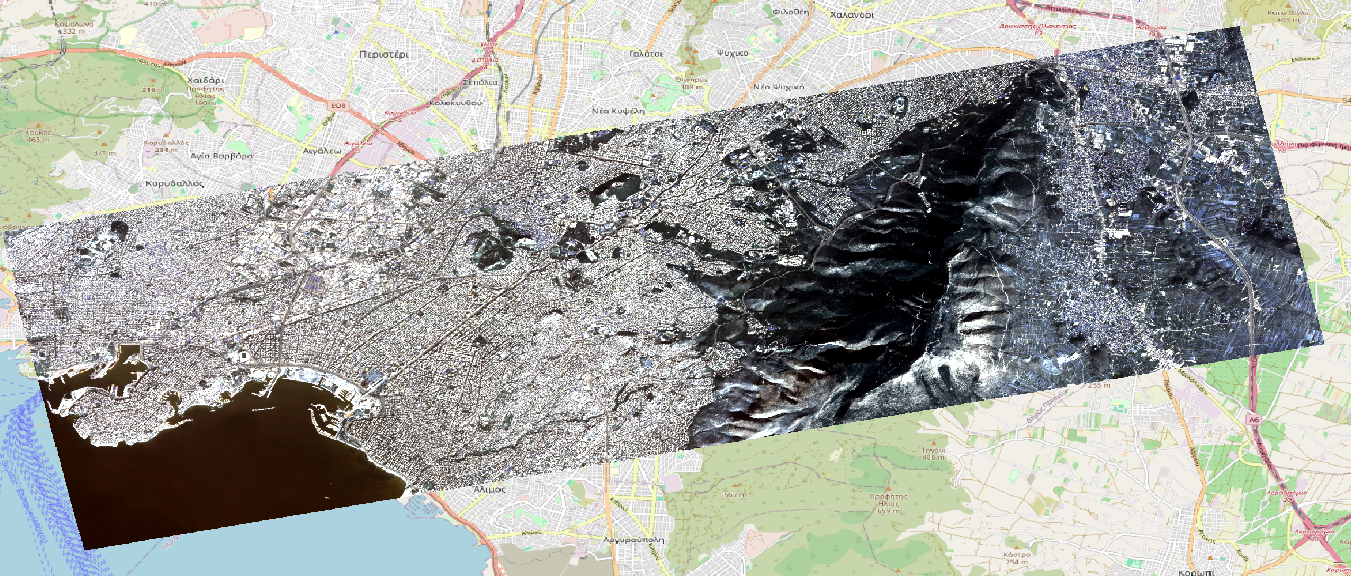
\includegraphics[width=1\linewidth]{athens_greece_satimage.png}
    \caption{Satellite Image of Athens Greece, taken 31 January 2018. Imagery \textcopyright Planet Labs PBC 2023. All rights reserved.}
    \label{fig:athens_baseimage_ch2}
\end{figure}

\begin{table}
    \centering
    \begin{tabular}{|l|c|c|c|}
        \hline
            & \textbf{Dove Classic} & \textbf{Dove-R} & \textbf{SuperDove}\\
            \hline
         Band  & Wavelength (nm) & Wavelength (nm) & Wavelength (nm) \\
         \hline
         Red   & 590 - 670       & 650 - 682       & 650 - 680\\
         Green & 500 - 590       & 547 - 585       & 547 - 583\\
         Blue  & 455 - 515       & 464 - 517       & 465 - 515\\
         \hline\hline
         Image Area &  25 x 11.5 sq km & 25 x 23 sq km &32.5 x 19.6 sq km\\ \hline
         Availability & July 2014 - April 2022 & March 2019 - April 2022 & March 2020 - present \\ \hline
         
    \end{tabular}
    \caption{Technical Data from Planet about Planetscope\citep{planetScope}. As the Planetscope satellites have increased their capabilities over time, the technical specifications have slightly shifted.  Later generations of the satellites have more bands available, but to maintain continuity over our data set, we are only considering RGB bands. }
    \label{tab:planetscope_ch2}
\end{table}

\section{Convolutional Modeling}
Computer vision is a branch of machine learning that attempts to train computers to visually learn and identify objects similar to vision in humans \citep{goodfellow2016deep}.  Early attempts in this field were pioneered by Rosenblatt using perceptrons to attempt to identify letters visually \citep{rosenblatt1957perceptron}.  These early concepts, like perceptron, would develop and advance towards modern applications and the various forms of Deep Neural Networks \citep{fradkov2020early}.  These neural networks were not limited to a single perceptron or neuron, but could have many layers with complex connections among the layers.  Computational power and speed has improved significantly since the 1950s \citep{nordhaus2001progress}, and so has the advancement of neural networks.  

In this study, we rely on convolutional neural networks (CNN), a type of deep learning that is designed for the analysis of image data. These techniques have been shown to be effective at detecting, labeling and differentiating objects \citep{simonyan2014very, zhang2016deep, he2016deep, krizhevsky2017imagenet, voulodimos2018deep}.  CNNs represent a family of deep learning techniques that implement convolutional layers that extract features from an image \citep{zhang2016deep}.  There are many types of CNN architectures that have performed well across a wide range of computer vision tasks \citep{voulodimos2018deep,simonyan2014very,szegedy2015going}.  In general, convolutional networks refer to functions that take image inputs and kernels to generate outputs known as feature maps \citep{goodfellow2016deep}.  A formal definition is shown in formula \ref{cnn_def}.  The feature map, $\ S(i,j)$, is the output of image \textit{I} with dimensions \textit{i,j}, convolved with kernel \textit{K} with dimensions \textit{m,n} \citep{goodfellow2016deep}.  

\begin{equation}
S(i,j) = (K * I)(i,j) = \sum_{m} \sum_{n} I(i-m,j-n)K(m,n) 
%\caption{Formal definition of a convolution.  The feature map , $\ S(i,j)$, is the output of image \textit{I} with dimensions \textit{i,j}, convolved with kernel \textit{K} with dimensions \textit{m,n} \citep{goodfellow2016deep}.  }
\label{cnn_def}
\end{equation}

An early CNN  that leveraged GPUs was AlexNet \citep{krizhevsky2017imagenet}.  The architecture of AlexNet comprises five convolutional layers and three fully connected layers. Despite its relatively shallow structure, this network exhibits exceptional performance and played a crucial role in promoting the adoption of CNNs in computer vision. Notably, advancements in AlexNet demonstrated that the integration of dense convolutional layers could enhance performance \citep{szegedy2015going}.  A diagram of the architecture of AlexNet is displayed in figure \ref{fig:alexnet_architecture}.  

\begin{figure}
    \centering
    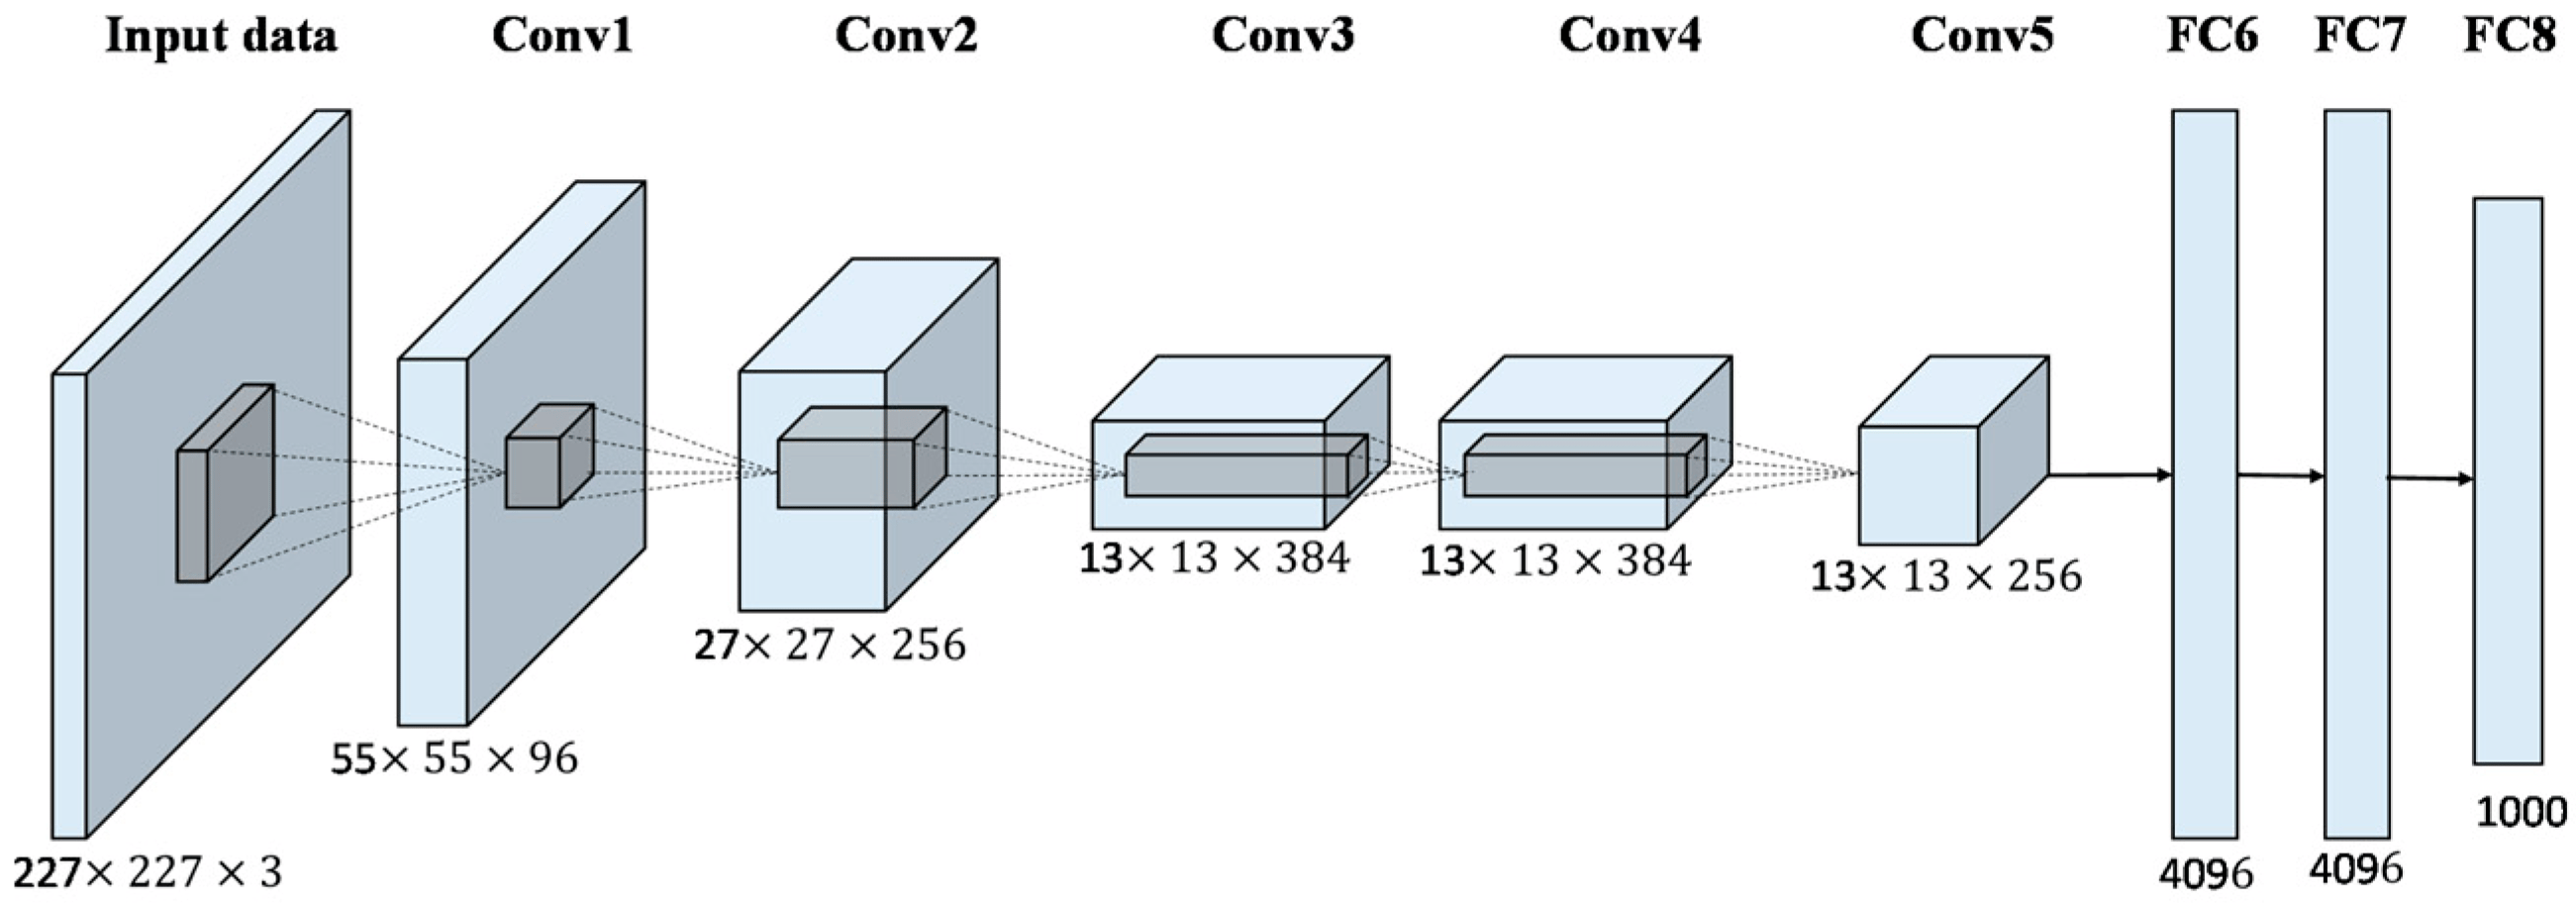
\includegraphics[width=0.5\linewidth]{Figures/alexnet_architecture.png}
    \caption{Architecture of AlexNet, highlighting input data passing through five convolutional layers and 3 fully connected layers.  Figure is from \citep{han2017pre}.}
    \label{fig:alexnet_architecture}
\end{figure}

Building upon this progress, a novel CNN named VGG was introduced by the vision geometry group at the University of Oxford \citep{simonyan2014very}. The VGG architecture emphasizes stacked convolutional layers with smaller kernel sizes, departing from individual convolutional layers with larger kernels. This approach yields significant computational gains and enables a more discriminative decision function through heightened non-linearity. Subsequent modifications and refinements to the VGG implementation have further improved the architecture's performance \citep{hu2018squeeze}.  A diagram of VGG is shown in figure \ref{fig:vgg_architecture}.

\begin{figure}
    \centering
    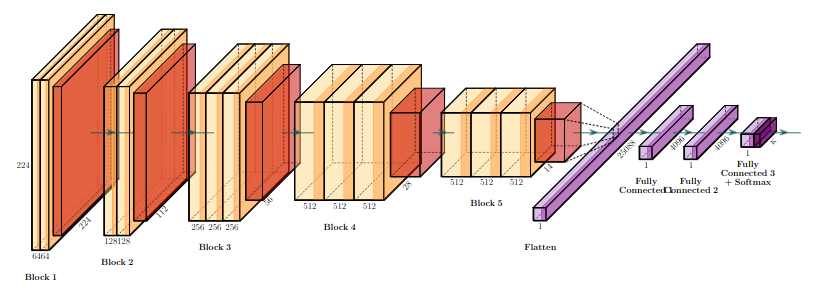
\includegraphics[width=0.5\linewidth]{Figures/vgg_architecture.png}
    \caption{Architecture of VGG, highlighting input data passing through stacked convolutional layers before flattening and passing through fully connected layers.  Figure is from \citep{vrbancic2019transfer}.}
    \label{fig:vgg_architecture}
\end{figure}

As VGG was developed, a desire to test so-called `deeper' networks took hold as a potential route forward for improved levels of capability \citep{simonyan2014very}.  However, VGG, AlexNet, and other earlier networks were functionally limited in the depth they could achieve due to - at the time - the difficulty of optimizing deep networks due to vanishing gradients \citep{he2016deep}.  ResNet, short for residual convolutional neural network, was developed to address the challenges associated with deeper networks while aiming to improve accuracy. A notable characteristic of ResNets is the inclusion of residual connections, which establish a direct path from one layer to deeper layers, bypassing intermediate convolutions (see figure \ref{fig:residual_block}). By incorporating these residual connections, the network can increase in depth without encountering issues related to gradient back propagation during optimization \citep{he2016deep}. Following the initial introduction of ResNets by He et al., subsequent researchers have made various improvements and modifications, often altering specific dimensions while preserving the general ResNet structure \citep{xie2017aggregated,zagoruyko2016wide}. Furthermore, others have explored alternative approaches to enhance the training process or optimize the loss functions employed in ResNets \citep{he2016identity,huang2016deep,he2019bag,wightman2021resnet}. The concept of forwarding information through skip connections has also been expanded into fully connected dense blocks in the DenseNet architecture \citep{huang2017densely}. Due to their remarkable effectiveness, ResNets have emerged as one of the dominant CNN architectures widely employed in contemporary deep learning applications.

\begin{figure}
    \centering
    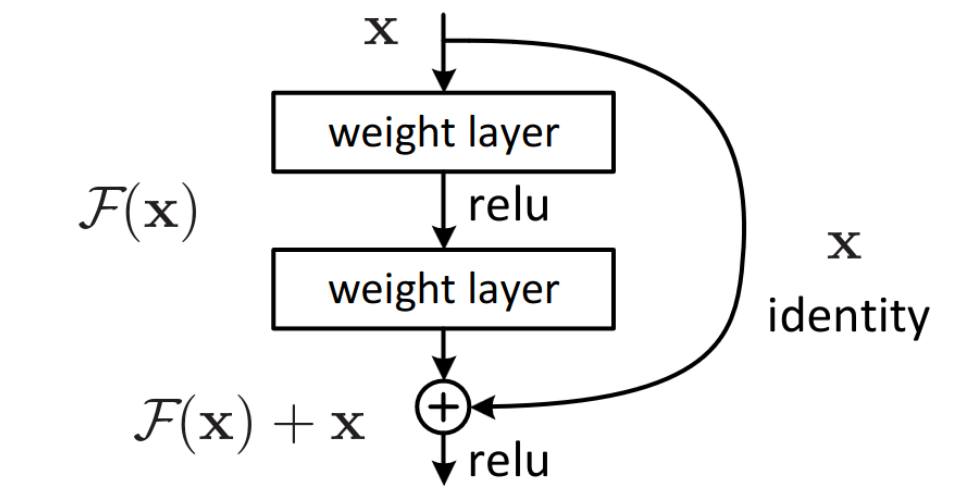
\includegraphics[width=0.5\linewidth]{Figures/residual_learning_block.png}
    \caption{Residual learning block, highlighting information flow deeper into networks that by passes itermediate layers.  Figure is from \citep{he2016deep}.}
    \label{fig:residual_block}
\end{figure}


\begin{figure}
    \centering
    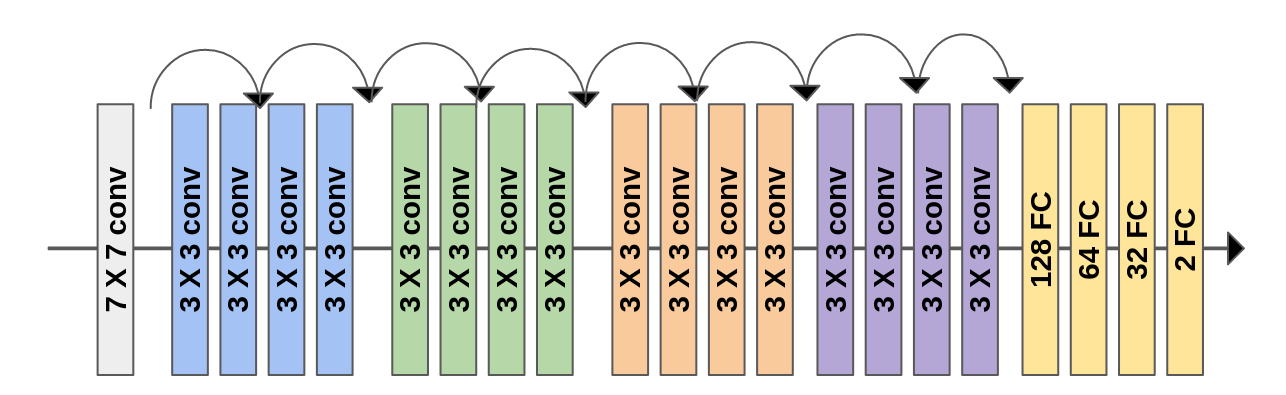
\includegraphics[width=1\linewidth]{Figures/resnet18_architecture.png}
    \caption{ResNet18, highlighting stacked convolutional layers, with residual learning depicted between intermediate convolutional layers.}
    \label{fig:resnet18_ch2}
\end{figure}

By 2016, ResNet architectures reached depths of 1001 layers, and achieved error percentages as low as 4.62\% on CIFAR-10 and 22.71\% on CIFAR-100 \citep{xie2017aggregated}.  Research has demonstrated ResNet-18's ability to identify cancer from x-ray images with 84\% accuracy \citep{khan2018evaluating}.  Various ResNet architectures have demonstrated the ability to semantically segment satellite imagery with accuracy over 80\%, depending on the specific architecture \citep{heryadi2020effect}.  While it is accepted that deeper neural networks tend to perform better under some circumstances \citep{he2016deep, lodhi2019multipath, sinha2020d2rl}, there can be benefits to using a shallower networks in some scenarios \citep{sekiyama2018profile,gorban2020deep}. 


\section{Explainability}

It is not uncommon for deep neural networks to be refereed to as "black boxes" \citep{dabkowski2017real,fong2017interpretable,petsiuk2018rise,chattopadhay2018grad,naidu2020cam}, due to the challenge of understanding why a model performs the way it does.  This is a particularly notable challenge in the field of computer vision, where an algorithm may leverage unexpected features to distinguish between cases \citep{wei2018deep}. 
\par
There have been multiple attempts to provide semantically-interpretable descriptions of what features are most important within a target image; these include analyzing intermediate convolutional layers \citep{zeiler2014visualizing}, inverting convolutional networks to understand image salience \citep{mahendran2015understanding,dosovitskiy2016inverting}, and Class Activation Mapping (CAM) \citep{zhou2016learning}.  Grad-CAM, introduced in \citep{selvaraju2017grad}, was able to generalize CAM for use in more deep learning models, by analyzing the gradients in the last convolutional layer to create a visualization indicating what regions in the original image are important for classification.  An example of Grad-CAM is displayed in figure \ref{fig:gradcam_introduced}.

\begin{figure}
    \centering
    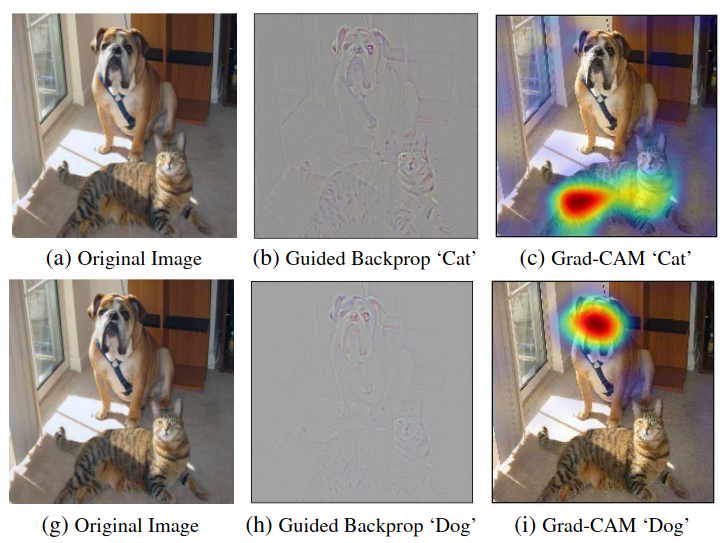
\includegraphics[width=0.5\linewidth]{Figures/gradcam_example.png}
    \caption{Images displaying the results of Grad-CAM analysis.  This example shows the ability of CAM techniques to highlight the relevant portion of images used in classification.  Image taken from \citep{selvaraju2017grad}}
    \label{fig:gradcam_introduced}
\end{figure}

Grad-CAM has lead to numerous variations with various benefits for specific scenarios.  Grad-CAM++ is an attempt to provide better localization of objects in the scene for classification \citep{chattopadhay2018grad}.  Score-weighted CAM (Score-CAM) is a variant that avoids using gradients, and instead uses weights to determine importance in the image \citep{wang2020score}.  Score-CAMpp uses logarithmic transformation in an attempt to reduce non-target information, providing a more focused map \citep{shi2022score}.  SSGrad-CAM is a spatial sensitive version of Grad-CAM that improves on object localization \citep{yamauchi2022spatial}.  Finally, Integrated Grad-CAM uses path integrals to better understand the regions of importance in a class activation mapping \citep{sattarzadeh2021integrated}.

Today, scholarship that explores the topic of explainability in the context of satellite imagery is sparse. Making the topic at hand more challenging, these past pieces have largely focused on discrete-case identification - for example, classifying well-defined semantic objects such as "airports", and identifying if the model identifies features such as "airplanes" \citep{vasu2018aerial,charuchinda2019use,fu2019multicam}.  This goal is distinct from the one posed by this dissertation, in which we seek to understand multiple urban features that may be correlated with an ill-defined semantic object (`protests' or `riots'). This is challenging because of the following gaps in the literature:
\textbf{1.} There are multi-target limits in exlainability techniques developed in conjunction with object based images.
\textbf{2.} Satellite imagery is inherently less variable in band-space than other types of images.
\textbf{3.} It is not immediately clear what is and is not semantically useful in satellite imagery-based classification.

The first key gap is multi-target limits on existing methods.  These are cases in which multiple, discrete features that are not contiguous may be important to classification to different degrees.  For example, object detection in satellite imagery can struggle when there are many objects present, such as multiple airplanes at an airport \citep{tahir2022automatic}.  Existing models struggle with this because often times the scale of objects in satellite imagery are smaller than objects in traditional images \citep{tahir2022automatic} or if the model uses gradients to determine importance, the gradient can be relatively noisy \citep{wang2020score}.

The second challenge is in variability in band-space.  Unlike traditional images, satellite imagery often has limited variability in pixel values \citep{carleer2005assessment}.  Due to the correlative nature of the spatial information present in geographic data, this variability can be overcome with higher resolution. However, with the introduction of increased resolution, segmentation can become more challenging \citep{carleer2005assessment}.  Furthermore, the band range in visible colors is smaller in satellite imagery, when compared to traditional images \citep{brewer2022susceptibility}.  Having fewer differences in the imagery makes explaining the important features in the image more difficult.

The third difference is semantic utility.  In traditional image recognition space, the semantic definitions of object are often well understood - i.e., the ear of a cat is easily interpret-able.  In our context, a group of pixels that overlap a building, road and nearby park may be highlighted, leading to potential confusion over which feature (the building, road, or park) or combination of features was important to classification.  An example of this might be only having a few pixels to available to detect and label an airplane \citep{tahir2022automatic}, as opposed to having many pixels extract features that can assist in classifying fish species \citep{rodrigues2010automatic}. 



To overcome these limitations, in this dissertation, I propose to build on the capabilities of a technique called Score-CAM \citep{wang2020score}.  Score-CAM is a CAM method that attempts to explain, with a human interpret-able visual display, the features within an image that determine classification.  Score-CAM differs from traditional CAM methods that utilize gradients, and instead uses the forward pass scores of activation maps to determine the significance for target classes\citep{wang2020score}.  When masking the highlighted portions of CAM results, Score-CAM only decreased 31.5\% in predicted probability of the target class, compared to 47.8\% and 45.5\% decreases in GradCAM and GradCAM++ respectively \citep{wang2020score}.  This average drop percentage illustrates Score-CAM's improved ability to correctly identify the portions of the image that are most pertinent to classification.  Similarly, if the areas outside the CAM results are masked, Score-CAM increased in classification confidence by 30.6\%, while GradCAM and GradCAM++ only increased by 19.6\% and 18.9\% respectively \citep{wang2020score}.  This average increase percentage demonstrates Score-CAMs ability to focus on relevant portions of the image, not regions that do not assist in classification. For the purposes of this work, Wang et. al. found that it outperforms other techniques when there are multiple objects in a scene \citep{wang2020score}.  Score-CAM was selected as a baseline model to develop further due to its ability to handle multiple objects, and our data are satellite images which are scene-centric, containing multiple objects.  A figure displaying an example from the paper that introduced Score-CAM is shown in figure \ref{fig:scorecam_introduced}.

\begin{figure}
    \centering
    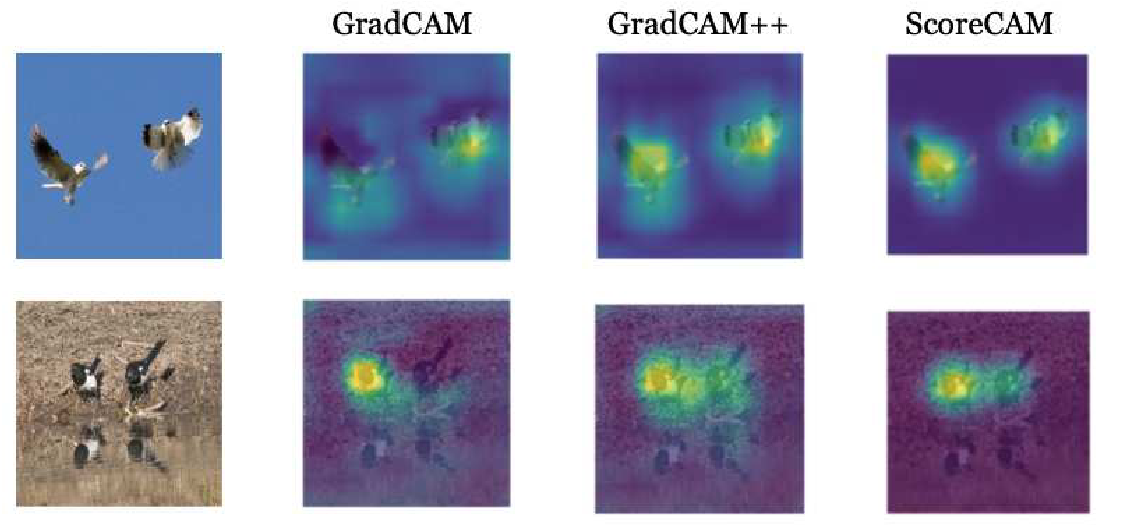
\includegraphics[width=0.5\linewidth]{Figures/scorecam_introduced_example.png}
    \caption{Images displaying the results of Score-CAM analysis.  This examples highlight the performance of Score-CAM when there are multiple objects from a given class present in the image.  Image taken from \citep{wang2020score}}
    \label{fig:scorecam_introduced}
\end{figure}









% Chapter Template

\chapter{Quantitative Analysis} \label{sec:chapter3} % Main chapter title
%this should end up being roughly 15-20 pages


\label{Chapter3} % Change X to a consecutive number; for referencing this chapter elsewhere, use \ref{ChapterX}

%----------------------------------------------------------------------------------------
%	SECTION 1
%----------------------------------------------------------------------------------------


\section{Data \& Methods}
The primary objective of this work is to predict if a riot or protest will occur in a specific urban area, based solely on data from satellite imagery.  In order to accomplish this objective, we leverage convolutional neural networks in combination with two data sources, ACLED \citep{ACLED} and Planet \citep{planet}. We use these data to generate two different sets of information: the first set is satellite imagery of locations where riots occurred, and the second is a set of images of proximate areas (within the same city) that did not experience a riot event.  Our deep learning model then seeks to disambiguate between these two cases, based on satellite imagery alone. This section provides details of our data processing and analytic approach.

\subsection{Data} \label{sec:data_paper1}
\subsubsection{Selecting Riot Locations}
Determining the locations where riots and protests have occurred is the first step in developing a data set for this work.  To identify these locations, we leverage the Armed Conflict Location Event Data Project (ACLED), an open source database which contains information on a wide range of conflict types from across the globe \citep{ACLED}.  ACLED contains more than 1.5 million events from 1997 to 2023, which are aggregated, categorized, and curated to create a data source that can specify time and location for conflict.  We filter this database according to a number of criteria:
\begin{enumerate}[topsep=0pt,itemsep=-1ex,partopsep=0ex,parsep=0.5ex]
\item \textbf{Type of event. } We focus our analysis on protests and riots, which primarily represent urban unrest.
\item \textbf{Date. } We only leverage protest or riot events with a known date of occurrence.
\item \textbf{Geography. } Only events with a known neighborhood-level geographic footprint are selected.\footnote{For example, some riots are known to have occurred in Beriut, while others occurred within neighborhoods in Beriut. There are 12 neighborhoods listed within some of the ALCED entries for Beriut (Ras Beirut, Port, Mazraa, Achrafieh, Mousseitbeh, Saifi, Minet El Hosn, Rmeil, Bachoura, Medawar, Ain Mreisseh, and Zokak El Blat).  These neighborhood specific entries have neighborhood specific latitudes and longitudes, and we use these neighborhood specific events to construct our data set.}
\end{enumerate}

After filtering events, we are left with a resultant database of 53,307 events. In order to prevent over representation of any single unique location in the database, a maximum of 500 events were randomly selected from each neighborhood (i.e., "Seoul - Jongno"). After this stage, a total of 37,728 events across 1,089 unique locations were leveraged to construct our dataset of the location of conflict events.






\subsubsection{Satellite Data}
Once we have identified the location of riot events, we retrieve relevant \textit{Planetscope} satellite imagery both (a) 24-48 hours prior to each event, and (b) in similar, nearby geographic locations that did not experience unrest.  Planetscope - an integrated collection of images from the Dove, Dove-R and SuperDove satellites - provides four-band (RGB and NIR), approximately three to four meter spatial resolution satellite imagery with a daily temporal resolution (\cite{planetScope}; see table \ref{tab:planetscope}). For both cases of imagery (with and without riot), we consider images that contain less than 50\% cloud cover.  An example of the imagery available can be seen in figure \ref{fig:athens_baseimage}.  


\begin{table}
    \centering
    \begin{tabular}{|l|c|c|c|}
    \hline
            & \textbf{Dove Classic} & \textbf{Dove-R} & \textbf{SuperDove}\\
         Band  & Wavelength (nm) & Wavelength (nm) & Wavelength (nm) \\
         \hline
         Red   & 590 - 670       & 650 - 682       & 650 - 680\\
         Green & 500 - 590       & 547 - 585       & 547 - 583\\
         Blue  & 455 - 515       & 464 - 517       & 465 - 515\\
         \hline
    \end{tabular}
    \caption{Technical wavelength specifications for RGB bands of Planetscope sensors \citep{planetScope}.  }
    \label{tab:planetscope}
\end{table}

\begin{figure}
    \centering
    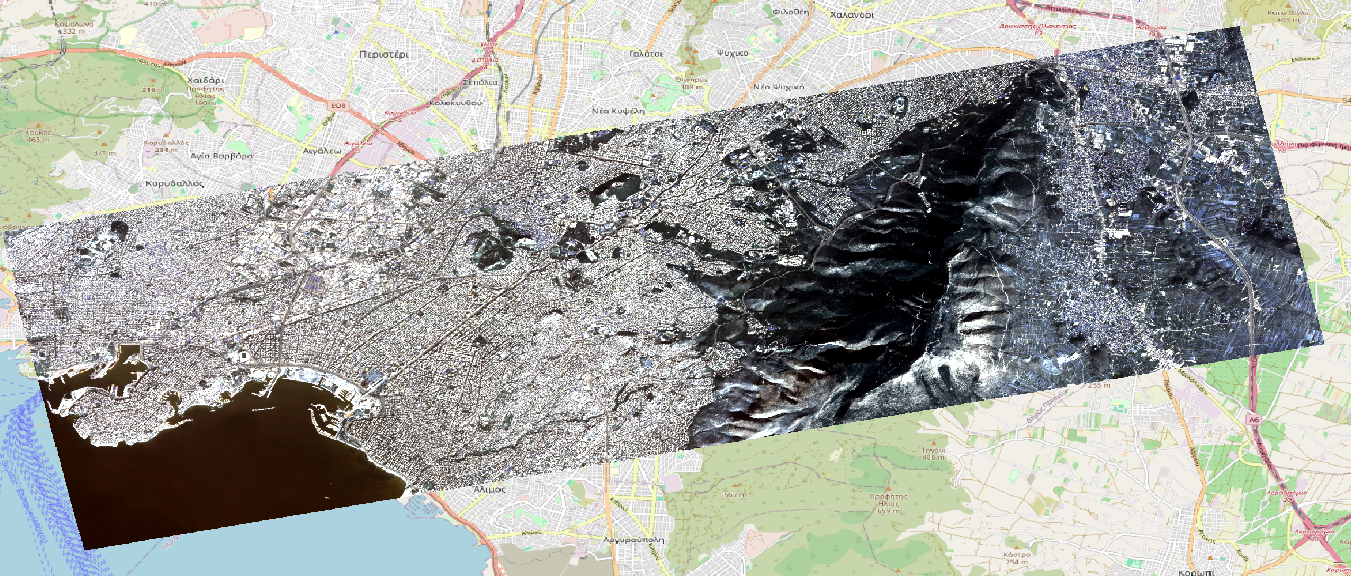
\includegraphics[width=1\linewidth]{athens_greece_satimage.png}
    \caption{Satellite Image of Athens Greece, taken 31 January 2018. Imagery \textcopyright Planet Labs PBC 2023. All rights reserved.}
    \label{fig:athens_baseimage}
\end{figure}


\begin{table}[htbp]
    \centering
    \caption{PlanetScope Constellation \citep{planetScope} }
    \begin{tabular}{|l|l|l|}
        \hline
        \textbf{Instrument} & \textbf{Image area} & \textbf{Availability} \\
        \hline
        Dove Classic & 25 x 11.5 sq km & July 2014 - April 2022 \\
        Dove-R & 25 x 23 sq km & March 2019 - April 2022 \\
        SuperDove & 32.5 x 19.6 sq km & March 2020 - present \\

        \hline  
    \end{tabular}
    \label{tab:doves}
\end{table}


For each of the 37,728 instances of riots in our filtered ACLED dataset, we first retrieve a full scene of imagery from 24-48 hours prior to the event.  These scenes are guaranteed to encompass the latitude and longitude representing the centroid of the neighborhood at which a conflict occurred; in cases where multiple images were available for a given event we chose the one closest in time to the event (with a minimum of 24 hours prior to the event).  Ultimately, this process resulted in 19,902 satellite scenes being downloaded, with an average spatial dimension that can vary depending on the generation of satellite (see table \ref{tab:doves}) and geographic latitude of collection. Because riots may occur at the same location, but at multiple points in time, some locations (i.e., a seat of government, culturally significant locations, etc) may appear in the database multiple times; the most common of these occurrences are summarized in table \ref{tab:occurrence}.


\begin{table}[htbp]
    \centering
    
    \begin{tabular}{|l|l|l|l|l|}
        \hline
        \textbf{Country} & \textbf{Neighborhood} & \textbf{Count} & \textbf{Earliest Date} & \textbf{Latest Date} \\
        \hline
        Pakistan & Karachi - Saddar &  278 & 7 October 2017 & 30 September 2022 \\
        Iran & Tehran - District 6 &  270 & 9 October 2017 & 26 September 2022 \\
        Iran & Tehran - District 12 & 268 & 9 October 2017 & 28 September 2022 \\
        Lebanon & Beirut - Port & 252 & 7 October 2017 & 26 September 2022 \\
        Greece & Athens - Central Athens & 247 & 18 January 2018 & 28 September 2022 \\
        South Korea & Seoul - Jongno &  240 & 18 January 2018 & 21 September 2022 \\
        South Korea & Seoul - Jung & 226 & 18 January 2018 & 26 September 2022 \\
        Italy & Rome - City Center &  222 & 7 January 2018 & 23 September 2022 \\
        India & Delhi - New Delhi &  220 & 2 October 2017 & 4 September 2022\\
        South Korea & Seoul - Seocho & 220 & 8 January 2018 & 28 September 2022 \\
        \hline
    \end{tabular}
    \caption{Neighborhood locations which occur most frequently.  `Earliest' and `Latest' date refer to the earliest and latest date of a protest event for each neighborhood.  For example, in the neighborhood of Seocho in Seoul, 220 independent protest or riot events occurred from January 8th, 2018 to September 28th, 2022.  In our analysis, this would be represented by 220 individual satellite tiles, each taken between 24 and 48 hours before the actual event.}
    \label{tab:occurrence}
\end{table}



From the satellite scene retrieved for each conflict event, we extract two types of data.  First, we extract a one kilometer by one kilometer box centered on the conflict event neighborhood.  This box is saved and identified as the location of the unrest in our database.

Second, we extract a number of cases to serve as null events - i.e., locations from the same urban area, but where no unrest occurred.  To generate these null cases, we follow a multiple step process in which we:

\begin{enumerate}[topsep=0pt,itemsep=-1ex,partopsep=0ex,parsep=0.5ex]
\item \textbf{Identify urban areas. } We only consider areas in the scene that have a population density over 300 inhabitants per kilometer.
\item \textbf{Exclude areas that are within 10km of the conflict event. } We isolate the conflict event by removing the urban areas that are within ten kilometers of the centroid of the neighborhood in which conflict occurred.
\item \textbf{Sample. } With the remaining urban areas in the satellite scene, we generate a list of random centroids which are constrained to be a minimum of 2 kilometers apart, and select a maximum of 10 of these to generate 1km box `null' locations at which no protest or conflict occurred.  The 2 kilometer separation ensures that none of our null boxes overlap.
\end{enumerate}


In step one, we overlay information about the degree of urbanization \citep{ghs_smod_2023, urbanisation_manual_2021} onto each satellite scene to determine what portions are urban, and which parts are not.  This is accomplished by using the DEGURB dataset \citep{ghs_smod_2023}, which was developed by the European Commission's Joint Research Centre.  This data categorizes geographical areas into Urban Centre, Urban Clusters (including towns and suburbs), and Rural Grid Cells (including villages and dispersed rural) zones based on population density and contiguity of dense areas \citep{urbanisation_manual_2021}.  Its creation involves analyzing high-resolution satellite imagery and detailed population survey data, with the goal of providing an accurate representation of the urban landscape with one kilometer spatial resolution \citep{urbanisation_manual_2021}. The DEGURB dataset used in this work is representative of 2020 \citep{ghs_smod_2023}.  For our purposes we consider anything with a density over 300 inhabitants per square kilometer as urban \citep{urbanisation_manual_2021}.   The results of this approach are illustrated in figure \ref{fig:degurb}.  This binary representation of urban areas is then be applied to each satellite scene as a mask, allowing us to select null cases from proximate urban areas.

\begin{figure}
    \centering
    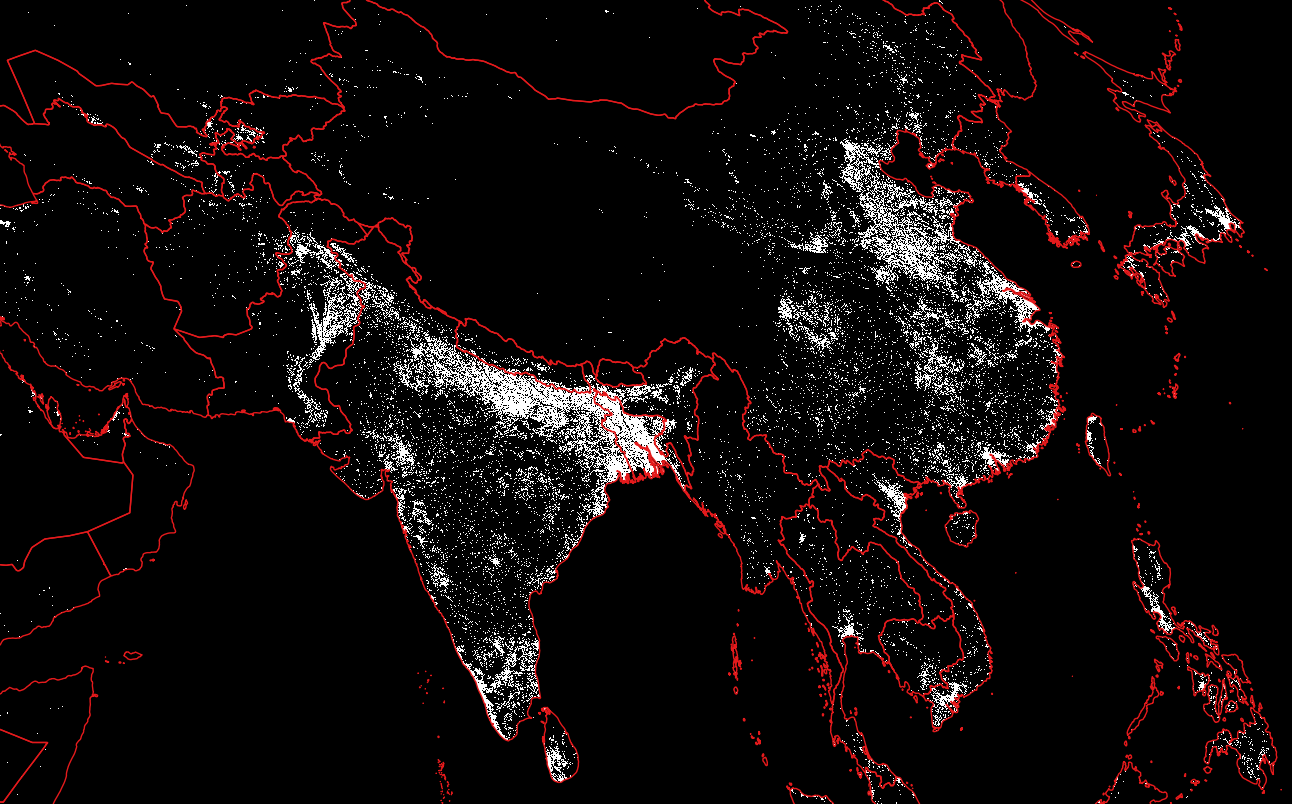
\includegraphics[width=0.9\linewidth]{degurb_B.png}
    \caption{A portion of the DEGURB data, highlighting areas of the world that are considered urban in our data set. DEGURB defines urban regions as those with a density more than 300 inhabitants per km \cite{urbanisation_manual_2021}.  Red lines represent country level boundaries \citep{runfola2020geoboundaries}.  }
    \label{fig:degurb}
\end{figure}


In step two, in order to ensure the areas selected for null cases are distinct from the areas of unrest, we exclude all urban areas up to 10 kilometers away from the centroid of the riot neighborhood from consideration, as illustrated in figure \ref{fig:athens_nullclips}.




Third, after excluding the ten kilometer region around each unrest event, from the remaining urban regions in the satellite scene we select random locations for null-riots.  We accomplish this by generating a list of random latitudes and longitudes that are within the available regions.  We ensure that each of these random locations are at least 2 kilometers away from any other locations on our random list.  We then take a maximum of ten of these locations, and construct a 1 kilometer box around each one.  We construct up to 10 null cases (that do not overlap) from the eligible urban regions from each scene (noting that less dense urban areas are occasionally represented by less than 10 null cases due to a lack of proximate urban areas). A visualization of the results from this process can be seen in figure \ref{fig:athens_nullclips}.

  

\begin{figure}
    \centering
    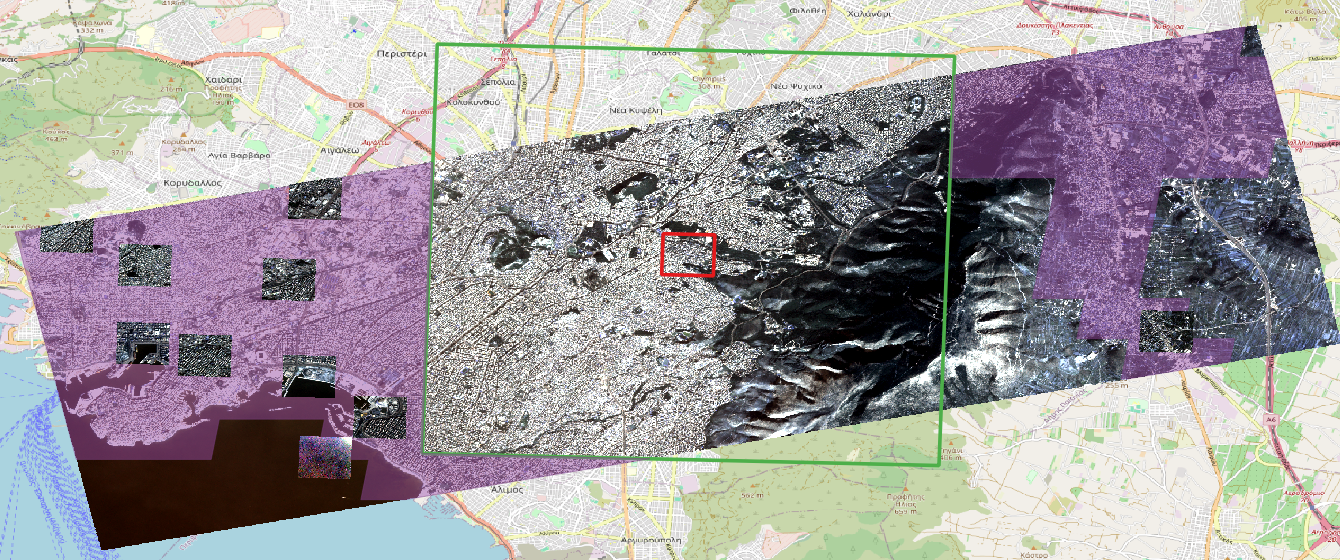
\includegraphics[width=0.9\linewidth]{athens_greece_nullclips.png}
    \caption{Satellite Image of Athens Greece, taken 31 January 2018.  The red box in the center of the image is a 1 kilometer box around the riot location.  The green box is a 10 kilometer exclusionary area around the riot location, from which we do not draw "null" case contrasts.  Areas which fall outside the green box, that are also urban, are eligible for selection (displayed  in purple).  From the potential null region, we sample random, non-overlapping 1 kilometer boxes to generate null location clips. Imagery \textcopyright Planet Labs PBC 2023. All rights reserved.}
    \label{fig:athens_nullclips}
\end{figure}



After this process is completed, for each conflict event we are left with a set of one ($\ 1 km^{2} $) kilometer box representative of where unrest occurred, and up to 10 ($\ 1 km^{2}$)  km boxes representative of urban areas proximate to the unrest event, but with no known activity.  Across our full dataset of 19,902 unrest locations, 18,634 (93.6\%) had 10 null cases available; the distribution of null cases across images can be seen in figure \ref{fig:null_hist}. Our final dataset included only locations that had the full complement of null clips, for a total of 18,631 cases of unrest, and 186,310 null cases. We then normalize all of these image clips based on a sample of the full satellite scenes \citep{goodman2021convolutional, runfola2022deep, lv2024mapping, brewer2023tracking}.  Tests of different permutations of this dataset (i.e., models with a 1:1 ratio of null and riot cases) can be found in section \ref{sec:limited_data_set}.



\subsection{Methods}\label{sec:methods_paper1}
Our overall modeling architecture is summarized in figure \ref{fig:flow_chart}. In order to estimate the likelihood of if an unrest event occurred or not at each location, we leverage a ResNet18 \citep{he2016deep} as our base model, replacing the fully connected layer with a series of dense layers with 128, 64, and 32 hidden nodes.  In order to improve the efficiency of our training, following other literature in the satellite imagery analysis space \citep{goodman2021convolutional, brewer2021predicting, runfola2022deep, lv2024mapping, brewer2023tracking}, pre-trained weights from ImageNet were used as our initial baseline. 

\begin{figure}
    \centering
    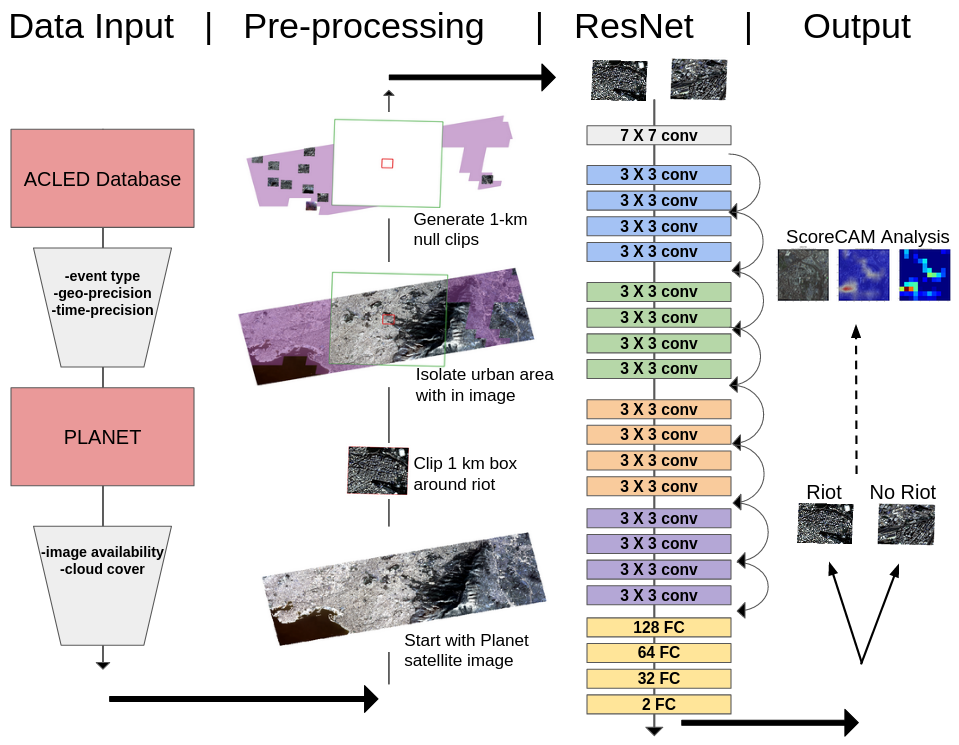
\includegraphics[width=0.75\linewidth]{flow_chart.png}
    \caption{A synopsis of our overall modeling architecture.  Stages include the collection of data, pre-processing, network training, categorization, and explainability analysis. Imagery \textcopyright Planet Labs PBC 2023. All rights reserved.}
    \label{fig:flow_chart}
\end{figure}

\subsubsection{Hyperparameter Search}
Prior to training on all 18,631 images, we first randomly selected a subset of 1,000 conflict events (1,000 unrest cases and 10,000 null cases) to implement a grid search across hyper-parameters \footnote{Training was performed using pyTorch on 8 RTX 6000 NVIDIA GPUs.  On average, models trained using the hyperparameter dataset took approximately 6.5 hours to complete 40 epochs; our full model across all images took 321 hours for 100 epochs.}. To account for class imbalance, we implement a weighted cross entropy loss \citep{ho2019real} with an ADAM optimizer \citep{kingma2014adam} for our training procedure.  

Our hyperparameter search encompassed trials of different learning rates, L2 regularization, dropout, freezing layers (results and parameters from a sample of the trials can be seen in the appendix in section \ref{large_table_of_results}).  Results from a selection of three of the best performing cases in the hyperparameter testing are shown in table \ref{tab:hyper_param_search}. On the basis of these results, we selected one model (denoted as Model C in table \ref{tab:hyper_param_search}) to test on the full dataset, which is described in table \ref{tab:fulldata_results_table}.
\par
We assess our model by interpreting the overall accuracy, precision and recall.  The precision is the ratio of true positives to the number of positive predictions our model made \citep{davis2006relationship}, which will measure our model's ability to correctly predict riots when it does makes a prediction.  The recall is the ratio of true positives to the number of riots in the data set, which measures our model's ability to identify how frequently riots are occurring \citep{davis2006relationship}.  

\begin{table}
\centering
\resizebox{\textwidth}{!}{%
\begin{tabular}{|l|p{1.5cm}|p{1cm}|p{2cm}|p{1.5cm}|p{1cm}|p{1cm}|p{1cm}|p{1cm}|p{1cm}|p{1.5cm}|p{1.5cm}|p{1.5cm}|}
    \hline
    Model & \raggedright Learning Rate & L2 Decay & \raggedright Freeze Layers & Drop Out & \raggedright Test Acc & TP & FP & FN & TN & Precision & Recall & F1 \\
    \hline
    A & 0.000001 & None & None & No & 92.5\% & 56 & 34 & 122 & 1,861 & 62.2\% & 31.5\% & 41.8\% \\
    B & 0.000015 & 0.01 & First 5 & No & 90.5\% & 95 & 103 & 93 & 1,782 & 48.0\% & 50.5\% & 49.2\% \\
    C & 0.00001 & 0.001 & First 5 & No & 92.2\% & 95 & 55 & 107 & 1,816 & 63.3\% & 47.0\% & 54.0\% \\
    \hline
\end{tabular}%
}
\caption{Representative results from hyperparameter tuning efforts. All training iterations were based on the same ResNet18 architecture, training with the same 1,000 satellite images from the full dataset, for 40 epochs. }
\label{tab:hyper_param_search}
\end{table}



\subsubsection{Additional Analyses} \label{sec:validation_methods}
In addition to identifying the best convolutional model performance, we additionally implement two additional analyses to better understand the strengths and weaknesses of this approach.  These include (a) generating information on the country-level performance of the model, and (b) and explanatory model that sought to identify the features within a given image that were correlated with conflict events (or the lack thereof).  
\par
To explore the spatial distribution of accuracy of the approach, we first filter our data to only consider countries that had 500 or more observations (a minimum of 250 riot clips and 250 null clips).  This created a validation set consisting of 32,548 clipped images, distributed across 24 countries (see table \ref{tab:val_data_selection}). From this, we withhold 20\% of each country's observations for validation after training.  This ensures that each country has at least 100 observations (50 riot clips and 50 null clips) for validation.  We then selected the hyperparameters from our best performing model (model C, see table \ref{tab:hyper_param_search}), and trained a ResNet18 using 80\% of the validation data (26,058 images, half riot or protest and half null) for 50 epochs.  We then used the withheld 20\% of images (6,490 images, half riot or protest and half null) to test for accuracy within each country.

To begin to explore the underlying drivers of model performance, we additionally take preliminary steps towards trying to assess what features the model may be identifying and using in predictions.  To implement this process, we leverage Score-CAM \citep{wang2020score}.  Score-CAM is a Class Activation Mapping (CAM) method that attempts to explain, with a human interpret-able visual display, the features within an image that determine classification.  Score-CAM differs from traditional CAM methods that utilize gradients, and instead uses the forward pass scores of activation maps to determine the significance for target classes \citep{wang2020score}.  For the purposes of this work, Wang et. al. found that it outperforms other techniques when there are multiple objects of relevance in the scene \citep{wang2020score}, a nearly universal characteristic of satellite imagery.  

\section{Results}

\subsection{Full Data Set}
In this section, we report our findings from our analysis of the full dataset (N= 204,941 clipped images), using the best performing model from our hyper-parameter testing (model C, as described in table \ref{tab:hyper_param_search}).  Results of this model are presented in table \ref{tab:fulldata_results_table}.  
\par
As table \ref{tab:fulldata_results_table} shows, the approach outlined in this paper achieve an overall accuracy of 97.39\% - i.e., of the 40,989 images in the test dataset, 39,921 were correctly identified in terms of if the image is likely to be the site of a protest event or not.\footnote{It is important to note that our data set is constructed in a manner that would result in relatively high test accuracy.  We have one riot and ten null riot clips per satellite scene.  This means that if our model predicted no riot for every clipped image, the model would be correct 90.9\% of the time.  Even given imbalance in the data set, our trained model achieves better results, accurately predicting riots and null riots over 97\% of the time.  Further explorations of the value of the model in the context of imbalance are described in section \ref{sec:limited_data_set} of the appendix.} There are 3,646 riot or protest images in the testing set and the model correctly identifies 2,741 of these, resulting in a recall score of 75.18\%.  This demonstrates the model's ability to distinguish riot/protest events from non-riot events.  The model predicts there will be a riot in 2,904 of the images and is only incorrect 163 times producing a precision score of 94.30\%.  In the context of our scenario, when the model predicts there will be a riot or protest in an image, it is correct over 94\% of the time. 




\begin{table}
    \centering
    \begin{tabular}{|l|l|}

        \hline
        \textbf{Test Accuracy}  & \textbf{97.39\%} \\
        \hline
        True Positives (predict riot) & 2,741 \\
        \hline
        False Positives & 163 \\
        \hline
        False Negatives (missed riot) & 905 \\
        \hline
        True Negatives & 37,180 \\
        \hline
        \hline
        Precision & 94.39\% \\
        \hline
        Recall & 75.18\% \\
        \hline
        F1 Score & 83.69\%  \\
        \hline
    \end{tabular}
    \caption{Results from ResNet18 using the full data set.}
    \label{tab:fulldata_results_table}
\end{table}



\begin{table}
\centering
\begin{tabular}{|l|l||l|l|}
\hline
\textbf{Country} & \textbf{Images} & \textbf{Country} & \textbf{Images}  \\ \hline
South Korea      & 7,494           & South Africa     & 1,480           \\ \hline
Pakistan         & 2,622           & Chile            & 1,302           \\ \hline
Iran             & 2,334           & Japan            & 1,256           \\ \hline
Lebanon          & 1,656           & India            & 1,148           \\ \hline
Palestine        & 1,572           & Brazil           & 1,112           \\ \hline
China            & 1,550           & Bangladesh       & 1,092           \\ \hline
\hline
\textbf{Country} & \textbf{Images} & \textbf{Country} & \textbf{Images} \\ \hline
Ukraine          & 924             & Greece           & 634          \\ \hline
Thailand         & 890             & Yemen            & 604           \\ \hline
Italy            & 728             & United Kingdom   & 566          \\ \hline
Indonesia        & 678             & Taiwan           & 562          \\ \hline
Russia           & 668             & Peru             & 522           \\ \hline
Venezuela        & 648             & Iraq             & 506           \\ \hline
\end{tabular}
\caption{There are 32,548 clipped images in the validation data set.  Half of these are from riots/protests, and half are null clips.  Only countries that have at least 500 images are included.  20\% of each county's images will be withheld from training and testing, and used in validation.}
\label{tab:val_data_selection}
\end{table}

In addition to the global accuracy, we also subset our data by country and report accuracy within each based on a validation set (see section \ref{sec:validation_methods} of our methods). The results of this country-specific validation testing are shown in table \ref{tab:validation_country_results}.\footnote{Of note, the re-trained model which withheld data for each individual country had a slightly lower global accuracy than our full results, of 89\%. While this 89\% accuracy is lower than the accuracy from the full data set shown in table \ref{tab:fulldata_results_table}, the testing circumstances of the validation are more challenging due to the even split between riot and null in the validation data set.  Additionally, there are known limitations in our images that likely contribute to a decrease in performace.  These limitations are discussed in greater depth in section \ref{sec:limits.satinfo}.  The precision and recall for the validation set were inline with the accuracy, each scoring slightly over 89\%.} Lebanon (94.5\%), Iran (94.4\%), and Pakistan (92.6\%) were the most accurate in this analysis, while Yemen (78.3\%), Russia (78.0\%), and Peru (77.9\%) were the least accurate countries.  No clear regional patterns existed, though some evidence suggests that accuracy and total number of observations may be correlated (i.e., less accurate news media reporting in Russia may be attributable to the lower accuracy in that context).

\begin{figure}
    \centering
    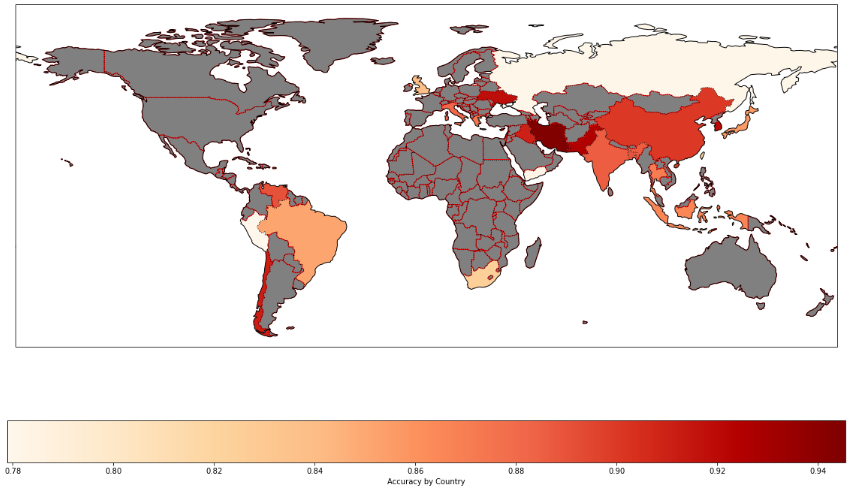
\includegraphics[width=0.75\linewidth]{Figures/global_accuracy_by_country.png}
    \caption{Map of 24 countries included in validation testing.  Each country in the validation testing has a minimum of 100 images.}
    \label{fig:global_map_validation}
\end{figure}


\begin{table}
    \centering
    \begin{tabular}{|l|l|}
        \hline
        \textbf{Test Accuracy}  & \textbf{89.41\%} \\  \hline
        True Positives (predict riot) & 2,903 \\       \hline
        False Positives & 345 \\   \hline
        False Negatives (missed riot) & 342 \\  \hline
        True Negatives & 2,900 \\  \hline
        \hline
        Precision & 89.38\% \\        \hline
        Recall & 89.46\% \\        \hline
        F1 Score & 89.42\%  \\
        \hline
    \end{tabular}
    \caption{Results from validation testing.}
    \label{tab:validation_global_results}
\end{table}



\begin{table}
\centering
\begin{tabular}{|l|l|l|l|l|l|l|}
\hline
\textbf{Country} & \textbf{Count}& \textbf{Accuracy} & \textbf{TP} & \textbf{FP} & \textbf{TN} & \textbf{FN} \\ \hline
Lebanon        & 330  & 94.54\% & 159 & 12 & 153 & 6  \\ \hline
Iran           & 466  & 94.42\% & 225 & 18 & 215 & 8  \\ \hline
Pakistan       & 524  & 92.56\% & 247 & 24 & 238 & 15 \\ \hline
South Korea    & 1498 & 92.12\% & 700 & 69 & 680 & 49 \\ \hline
Ukraine        & 184  & 91.85\% & 84  & 7  & 85  & 8  \\ \hline
Chile          & 260  & 91.15\% & 120 & 13 & 117 & 10 \\ \hline
Iraq           & 100  & 91.00\% & 45  & 4  & 46  & 5  \\ \hline
China          & 310  & 90.00\% & 140 & 16 & 139 & 15 \\ \hline
Palestine      & 314  & 89.49\% & 141 & 17 & 140 & 16 \\ \hline
Venezuela      & 128  & 89.06\% & 58  & 8  & 56  & 6  \\ \hline
Bangladesh     & 218  & 88.99\% & 90  & 5  & 104 & 19 \\ \hline
India          & 228  & 88.60\% & 97  & 9  & 105 & 17 \\ \hline
Italy          & 144  & 88.19\% & 62  & 7  & 65  & 10 \\ \hline
Greece         & 126  & 87.30\% & 62  & 15 & 48  & 1  \\ \hline
Thailand       & 178  & 87.08\% & 75  & 9  & 80  & 14 \\ \hline
Indonesia      & 134  & 86.57\% & 62  & 13 & 54  & 5  \\ \hline
Japan          & 250  & 85.60\% & 105 & 16 & 109 & 20 \\ \hline
Brazil         & 222  & 85.14\% & 94  & 16 & 95  & 17 \\ \hline
United Kingdom & 112  & 83.93\% & 50  & 12 & 44  & 6  \\ \hline
South Africa   & 296  & 82.43\% & 114 & 18 & 130 & 34 \\ \hline
Taiwan         & 112  & 82.14\% & 45  & 9  & 47  & 11 \\ \hline
Yemen          & 120  & 78.33\% & 41  & 7  & 53  & 19 \\ \hline
Russia         & 132  & 78.03\% & 50  & 13 & 53  & 16 \\ \hline
Peru           & 104  & 77.88\% & 37  & 8  & 44  & 15 \\ \hline
\end{tabular}
    \caption{Results from country level accuracy after validation testing.  These results are listed from highest accuracy to lowest accuracy.  We have also included the number of True Positives (TP), False Positives (FP), True Negatives (TN), and False Negatives (FN) for each country. }
    \label{tab:validation_country_results}
\end{table}

Of note, we observe a strong correlation between our softmax classification scores and accuracy within each country around the world, suggesting that softmax scores can be used as a proxy for prediction confidence (see figure \ref{fig:softmax_v_accuracy}).  While softmax may bias towards higher degrees of confidence \citep{pearce2021understanding, subramanya2017confidence}, as a relative metric it may provide helpful guidance to policymakers seeking to use these types of methods.

\begin{figure}
    \centering
    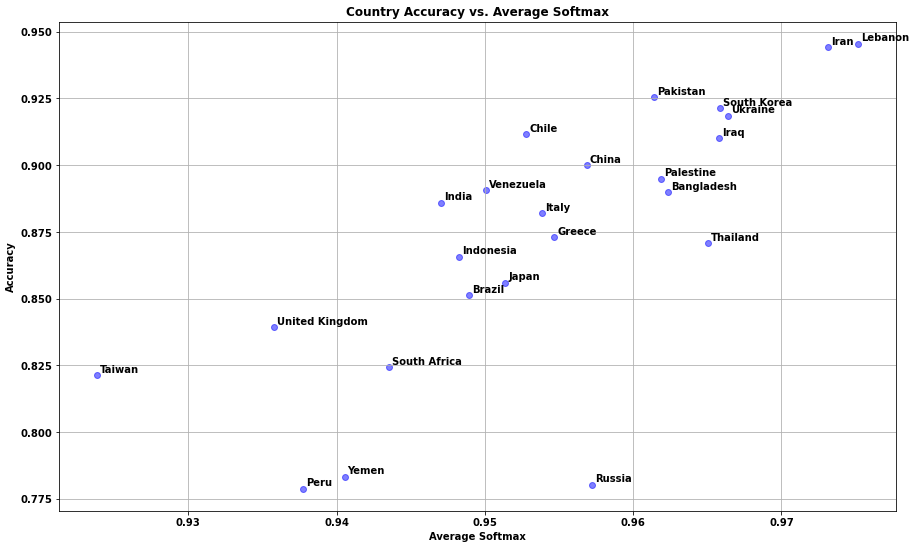
\includegraphics[width=0.75\linewidth]{softmax_v_accuracy.png}
    \caption{The average softmax for each country when compared to the average accuracy of prediction of each country.  Of note, the axis's do not begin at 0, but instead focus in on the domain and range of the values in the data.}
    \label{fig:softmax_v_accuracy}
\end{figure}


\subsection{Explainability of Results}

For our best performing model (model C in the table \ref{tab:fulldata_results_table}), we implemented Score-CAM on a subset of randomly selected, paired locations, ultimately consisting of 1,089 riot locations, and 1,089 null locations.  The Score-CAM results were then visually reviewed in an attempt to discern patterns in what the trained ResNet used in classification.  Interpreting the results of Score-CAM is inherently qualitative, making this a rich area for future work; we discuss this limitation further in section \ref{sec:explainability}.  
\par
Despite the limitations of Score-CAM, the visual interpretation indicated a few clear patterns.  An example of the first of these is displayed in figure \ref{fig:score_cam_stadium}, in which we can observe a large sports stadium in the image in the southeast region.  This large stadium is the location which Score-CAM identifies as the portion of the image which leads towards the classification (indicated through brighter values in the displayed heatmap).  In this case, the sports stadium lead the ResNet to classify the scene as a location that is unlikely to experience a riot.  We can see another example in figure \ref{fig:score_cam_stadium2}, in which again, the ResNet identifies the sports stadium as the reason to classify the scene as a non-riot.  We do not offer any explanation for why the sports stadiums are indicative of a non-riot scene, but these stadiums provide an example of the specific features which ResNet is learning to make classification decisions.  
\begin{figure}
    \centering
    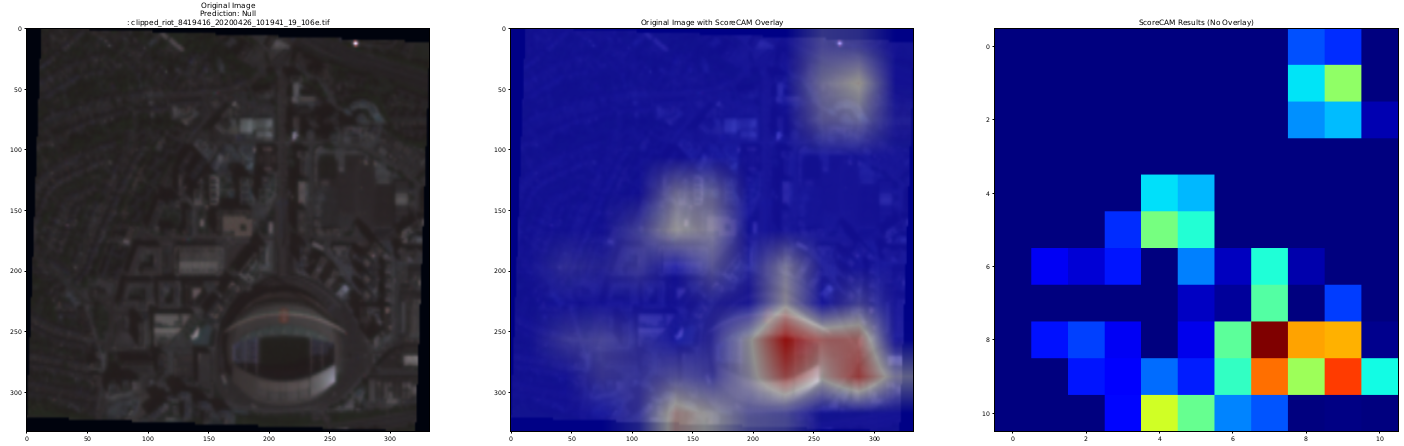
\includegraphics[width=1\linewidth]{scorecam_stadium.png}
    \caption{Example clipped image on the left.  The clipped image, a one kilometer box around a riot location.  The Score-CAM overlayed on top of the image is shown in the middle.  The Score-CAM visual is displayed on the right. Imagery \textcopyright Planet Labs PBC 2023. All rights reserved.}
    \label{fig:score_cam_stadium}
\end{figure}

\begin{figure}
    \centering
    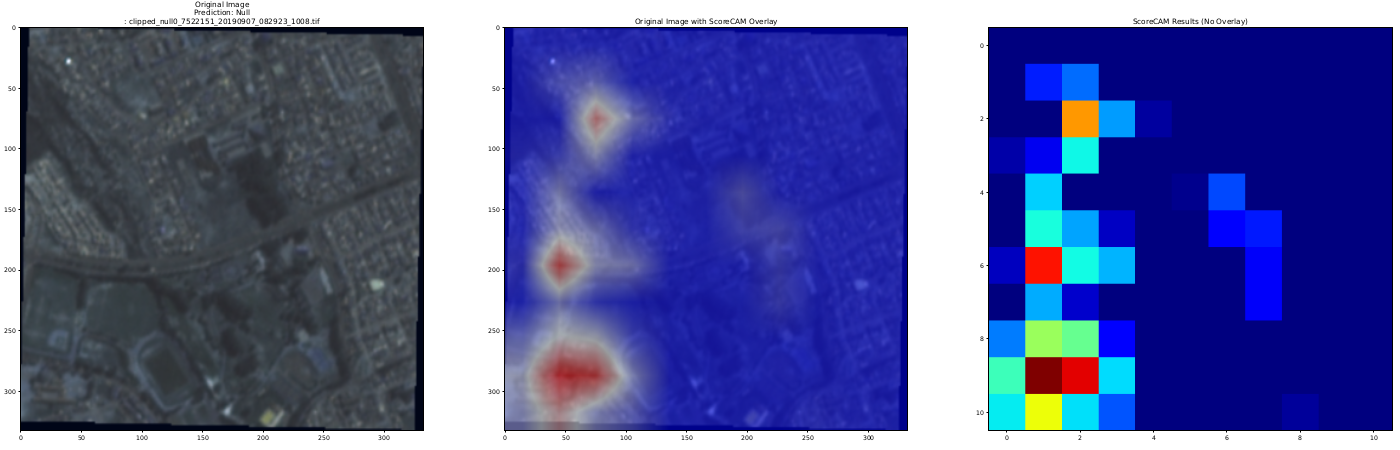
\includegraphics[width=1\linewidth]{stadium_scorecam2.png}
    \caption{Example clipped image on the left.  The clipped image, a one kilometer box around a non riot location.  The Score-CAM overlayed on top of the image is shown in the middle.  The Score-CAM visual is displayed on the right. Imagery \textcopyright Planet Labs PBC 2023. All rights reserved. }
    \label{fig:score_cam_stadium2}
\end{figure}

Another example highlighted in the Score-CAM analysis is shown in figure \ref{fig:fort_lalbagh}.  We can see a densely populated area, with a large open park or green space in the center of the image.  The trained network correctly predicted this image was from a riot or protest.  When we reference the ACLED data, this image is from a protest in the Lalbagh neighborhood of Dhaka, Bangladesh.  Lalbah is a fort built during the Mughal period in 1678, which was used subsequently by the British and Bangladesh governments as a location of governance and influence \citep{shakur2010culture}. Today, it is a location containing monument's and statues symbolizing rulers and regimes of the past, that is known as a common location for protests in the city of Dhaka \citep{begum2018changing}. While the deep learning model was not aware of these historic contexts, the unusual land use and associated image features were sufficient to classify this as a likely location of riots.

\begin{figure}
    \centering
    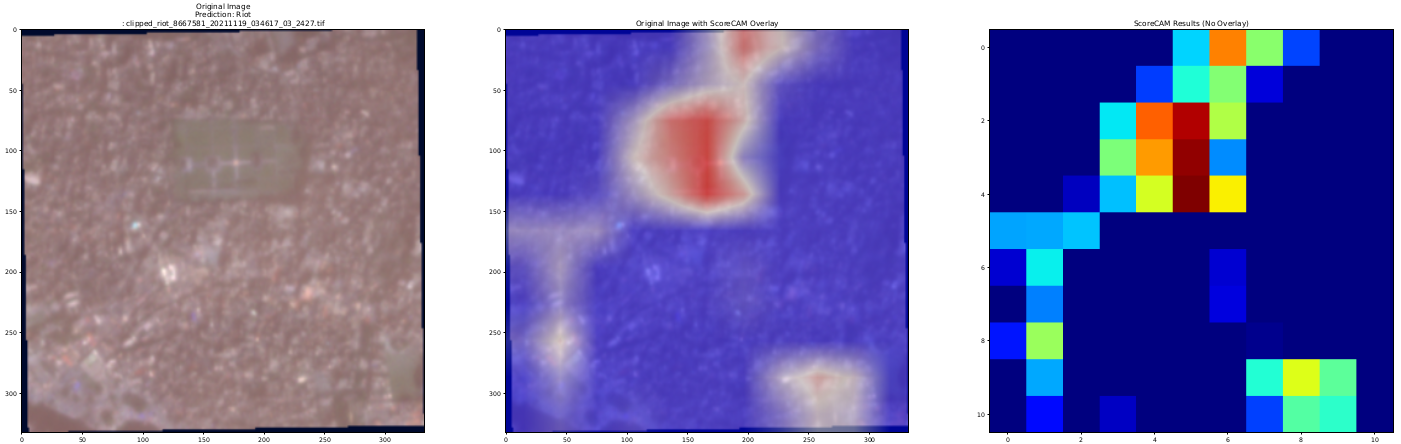
\includegraphics[width=1\linewidth]{fort_lalbagh_scorecam.png}
    \caption{The image on the left is a centered on Lalbagh Fort in Dhaka Bangladesh, taken on 19 November 2021, lesss than 48 hours before a protest at that location.  The Score-Cam visual is displayed on the right. Imagery \textcopyright Planet Labs PBC 2023. All rights reserved. }
    \label{fig:fort_lalbagh}
\end{figure}

\section{Discussion and Conclusions}
The results presented in table \ref{tab:fulldata_results_table} provide evidence that satellite information alone can provide useful information for the purposes of predicting where, within an urban environment, protests and riots are most likely to occur.  While this finding is likely to be of interest to those operating in data-sparse environments, it is well supported by past social science literature highlighting the interconnected nature of urban form and social processes \citep{fox2016urban,begum2018changing}.  By engaging in a global-scope study, here we are able to exploit this correlation by learning what these patterns are, and then leveraging them in estimation.  This finding held true across multiple model and data permutations (see tables \ref{tab:fulldata_results_table}, \ref{tab:validation_global_results} and \ref{tab:validation_country_results}), indicating that - even in some of the most challenging situations (i.e., relatively small training and validation sets), model accuracy can approach or exceed 90\%.

Furthermore, this technique performs well across the globe.  As highlighted in figure \ref{fig:global_map_validation}, there do not seem to be any regions that under perform.  Many countries with a relative low accuracy score (i.e., Russia) are in close proximity to a country with a higher accuracy score (i.e., China).  This pattern holds across the globe in South America, Asia, the Middle East, and Europe. 

Of note, in our softmax analysis seeking to correlate scores to accuracy, a single outlier, Russia, is observed in figure \ref{fig:softmax_v_accuracy} and table \ref{tab:validation_country_results}.  Russia has a lower comparative accuracy to other countries with similar softmax results.  This might be indicative of Russia's control of news sources \citep{gehlbach2010reflections}, or inherit bias in ACLED's collection of data which relies on news sources and non-governmental observation organizations that might not be focused on Russia.





\subsection{Conclusions}
In this work we constructed a data set consisting of 204,941 satellite images of riots and protests across the world.  After subseting the images into two classes of riots and non-riots, we trained a ResNet18 to identify which images were from locations associated with a riot.  When fine-tuned, our model achieved an accuracy of over 97\%, suggesting that satellite imagery has information of relevance and value to estimating the location of riot events.  This was true across a wide range of different tests and permutations of the data. We further provide some initial exploration into the explainability of this model, leveraging ScoreCAM to identify features the model is using in the classification task.


\section{Supplemental Information}\label{sec:appendix}



\subsection{Deduplication Tests}\label{sec:limited_data_set}

In this section, we present a test that controls for both class imbalance and geographic bias in our data. Our methodology leverages a large set of training data, specifically relying on an arbitrary 10:1 ratio of 10 null cases (no conflict event) to 1 positive case (a location where a conflict occurred).  Furthermore, some geographic locations are in the database multiple times - i.e., there may have been multiple protests at the same geographic location, even if they are at different dates (see table \ref{tab:occurrence}).  This results in both class imbalance (10 null cases for every 1 positive case), and geographic biases in where events are drawn from.  The class imbalance will potentially inflate accuracy scores, given a 10 to 1 ratio of null clips to riot clips - i.e., an untrained model could simply predict null for all images, and achieve an accuracy of 90.9\%.  Additionally, with repeated locations, the model will see the riot clip locations multiple times (i.e., even when each satellite scene has unique spatial information as it is drawn from a different date, the 1-km box centered on the latitude and longitude of the neighborhood will be the same).  This might allow our network to learn the specifics of a location, and over-fit to particular locations, instead of learning what features in urban areas predict riots and protests.  Therefore we constructed a limited data set to control for these issues.

To test if these attributes of our data resulted in bias, a new dataset was constructed which limited the data to a single riot image (1,089 1-km boxes) and a single non-riot image (1,089 1-km boxes) per location.  This means that our model was only able to analyze a riot location a single time during training, regardless of how frequently riots might happen at that location.  This should be a much harder training task for the model, with far less data available (2,178 images in total; these 2,178 images represent roughly 1\% of the data available for training in the full data set of 204,941 images).  Under these constraints, the maximum classification accuracy we observed was 67.37\% (see table \ref{tab:singleloc_results_table}).  Of note, the recall scores for our full data set and limited data set were very similar (75.18\% and 77.0\% respectively), despite the different size and scope of the training data.  

These results suggest that - even under extremely challenging, small-N circumstances - deep learning models can still identify meaningful features that are correlated with protest and riot events from satellite imagery.  


% Given the imbalance in our full data set, we also created a smaller data set without an imbalance.  In this smaller data set, there is only a single riot clip and single null clip per location.  We have also removed any repeated locations, creating a balanced data set with 1,089 riot clips and 1,089 null clips.  This is a more challenging scenario for training, because the model will only see each location a single time, and there is significantly less data available for training.  Even given the challenging scenario outlined, with this smaller data set the model performed well, achieving 65.57\% accuracy.  More detailed results can be seen in figure \ref{fig:singleloc_chart} and in table \ref{tab:singleloc_results_table}.  

% \begin{figure}
%     \centering
%     \includegraphics[width=0.5\linewidth]{singlelocation_finetuned.png}
%     \caption{Testing loss (in orange) and training loss (in blue) for the fine tuned model.  These results represent training the same fine tuned hyper parameter set, but only allowing a single riot clip and a single null riot clip per location.}
%     \label{fig:singleloc_chart}
% \end{figure}

\begin{table}
    \centering
    \begin{tabular}{|l|l|}
        \hline
        \textbf{Test Accuracy}  & \textbf{65.37\%} \\
        \hline
        True Positives (predict riot) & 154 \\
        \hline
        False Positives & 105 \\
        \hline
        False Negatives (missed riot) & 46 \\
        \hline
        True Negatives & 131 \\
        \hline
        \hline
        Precision & 59.46\% \\
        \hline
        Recall & 77.0\% \\
        \hline
        F1 Score & 67.1\%  \\
        \hline
    \end{tabular}
    \caption{Results from ResNet18 using only a single riot clip and single null riot clip per location.}
    \label{tab:singleloc_results_table}
\end{table}

\subsection{All Results} \label{large_table_of_results}
While we focus on our best performing models throughout this piece, there were a number of additional permutations and tests we performed while identifying the best modeling strategies, which we present here.  We began grid search across select hyperparameters, using a small test set of 100 random samples from our full data set.  Initially we were concerned with narrowing down the selection of the best performing learning rates, freezing layers of the ResNet, and dropping out connections between our fully connected layers.  The results of a sample of these are shown in table \ref{tab:initial_gridsearch_100A} and table \ref{tab:initial_gridsearch_100B}.  

\begin{table}
\centering
\begin{tabular}{|l|l|l|l|l|l|l|}
\hline
Metric & A1 & A2 & B1 & B2 & C1 & C2 \\ \hline
\hline
Test Accuracy (\%) & 91.59 & 91.12 & 90.65 & 93.93 & 93.46 & 86.45 \\\hline
\hline
True Positives & 0 & 0 & 0 & 0 & 0 & 0 \\ \hline
False Positives & 0 & 0 & 4 & 0 & 0 & 0 \\ \hline
False Negatives & 18 & 19 & 16 & 13 & 14 & 29 \\ \hline
True Negatives & 196 & 195 & 194 & 201 & 200 & 185 \\ \hline
\hline
Precision (\%) & 0.00 & 0.00 & 0.00 & 0.00 & 0.00 & 0.00 \\ \hline
Recall (\%) & 0.00 & 0.00 & 0.00 & 0.00 & 0.00 & 0.00 \\ \hline
F1 Score (\%) & 0.00 & 0.00 & 0.00 & 0.00 & 0.00 & 0.00 \\ \hline
\hline
Learning Rate & 1e-06 & 1e-06 & 1e-06 & 1e-06 & 1e-06 & 1e-06 \\ \hline
Freeze Layers & 0 & 0 & 5 & 5 & 10 & 10 \\ \hline
Drop Out Pair & (0, 0) & (0.1, 0.05) & (0, 0) & (0.1, 0.05) & (0, 0) & (0.1, 0.05) \\ \hline
L2 Weight Decay & 0 & 0 & 0 & 0 & 0 & 0 \\ \hline
\hline
\end{tabular}
\caption{All of the models in this table were tested with 100 random locations (100 riot clips and 1,000 null clips). In this table, all models used a learning rate of 1e-06. Models froze either none of the ResNet layers (A1, A2), the first 5 layers (B1, B2), or the first 10 layers (C1, C2). Between the first two and the second two layers, none of the connections were dropped (A1, B1, C1), or 10\% and 5\% were dropped (A2, B2, C2). }


\label{tab:initial_gridsearch_100A}
\end{table}



\begin{table}
\centering
\begin{tabular}{|l|l|l|l|l|l|l|}

\hline
Metric & D1 & D2 & E1 & E2 & F1 & F2 \\ \hline
\hline
Test Accuracy (\%) & 88.78 & 86.92 & 91.12 & 91.59 & 88.32 & 88.78 \\ \hline
True Positives & 5 & 1 & 7 & 5 & 0 & 0 \\ \hline
False Positives & 7 & 13 & 4 & 6 & 0 & 0 \\ \hline
False Negatives & 17 & 15 & 15 & 12 & 25 & 24 \\ \hline
True Negatives & 185 & 185 & 188 & 191 & 189 & 190 \\ \hline
\hline
Precision (\%) & 41.67 & 7.14 & 63.64 & 45.45 & 0.00 & 0.00 \\ \hline
Recall (\%) & 22.73 & 6.25 & 31.82 & 29.41 & 0.00 & 0.00 \\ \hline
F1 Score (\%) & 29.41 & 6.67 & 42.42 & 35.71 & 0.00 & 0.00 \\ \hline
\hline
Learning Rate & 1e-05 & 1e-05 & 1e-05 & 1e-05 & 1e-05 & 1e-05 \\ \hline
Freeze Layers & 0 & 0 & 5 & 5 & 10 & 10 \\ \hline
Drop Out Pair & (0, 0) & (0.1, 0.05) & (0, 0) & (0.1, 0.05) & (0, 0) & (0.1, 0.05) \\ \hline
L2 Weight Decay & 0 & 0 & 0 & 0 & 0 & 0 \\ \hline
\hline
\end{tabular}
\caption{All of the models in this table were tested with 100 random locations (100 riot clips and 1,000 null clips). In this table, all models used a learning rate of 1e-05. Models froze either none of the ResNet layers (D1, D2), the first 5 layers (E1, E2), or the first 10 layers (F1, F2). Between the first two and the second two layers, none of the connections were dropped (D1, E1, F1), or 10\% and 5\% were dropped (D2, E2, F2).}
\label{tab:initial_gridsearch_100B}
\end{table}

After the initial grid search, we increased the size of data set to 1,000 locations (1,000 riot clips, and 10,000 null clips).  We also adjusted the hyperparameter grid search space.  Our best performing model referred to as Model C in table \ref{tab:hyper_param_search}, is Config 10 in table \ref{tab:initial_gridsearch_1000B}.  Config 10 has the highest F1 Score across these grid search results, reflecting the best balance between Precision and Recall.  Due to this strong performance, these parameters were used to train the full dataset.


\begin{table}
\centering
\begin{tabular}{|l|l|l|l|l|l|l|}
\hline
Metric & Config 1 & Config 2 & Config 3 & Config 4 & Config 5 & Config 6 \\ \hline
\hline
Test Accuracy (\%) & 91.80 & 91.80 & 91.27 & 90.69 & 92.52 & 91.85 \\ \hline
True Positives & 62 & 39 & 43 & 77 & 25 & 78 \\ \hline
False Positives & 54 & 11 & 41 & 65 & 7 & 62 \\ \hline
False Negatives & 116 & 159 & 140 & 128 & 148 & 107 \\ \hline
True Negatives & 1,841 & 1,864 & 1,849 & 1,803 & 1,893 & 1,826 \\ \hline
\hline
Precision & 0.5345 & 0.7800 & 0.5119 & 0.5423 & 0.7812 & 0.5571 \\ \hline
Recall & 0.3483 & 0.1970 & 0.2350 & 0.3756 & 0.1445 & 0.4216 \\ \hline
F1 Score & 0.4218 & 0.3145 & 0.3221 & 0.4438 & 0.2439 & 0.4800 \\ \hline
\hline
Learning Rate & \multicolumn{6}{c|}{1e-05} \\ \hline
L2 Weight Decay & \multicolumn{3}{c|}{0.1} & \multicolumn{3}{c|}{0.01} \\ \hline
Freeze Layer & 0 & 0 & 0 & 5 & 5 & 5 \\ \hline
Dropout Pair & (0, 0) & (0.1, 0.05) & (0.5, 0.1) & (0, 0) & (0.1, 0.05) & (0.5, 0.1) \\ \hline

\end{tabular}
\caption{Model performance metrics for configurations 1 to 6 with learning rate of 1e-05, with variations in L2 weight decay, freeze layer, and dropout pair settings.}
\label{tab:initial_gridsearch_1000A}
\end{table}


\begin{table}
\centering
\begin{tabular}{|l|l|l|l|l|l|l|}
\hline
Metric & Config 7 & Config 8 & Config 9 & Config 10 & Config 11 & Config 12 \\ \hline
\hline
Test Accuracy (\%) & 91.51 & 89.77 & 92.91 & 92.33 & 90.16 & 92.76 \\ \hline
True Positives & 85 & 86 & 54 & 86 & 92 & 80 \\ \hline
False Positives & 64 & 106 & 34 & 32 & 101 & 49 \\ \hline
False Negatives & 112 & 106 & 113 & 127 & 103 & 101 \\ \hline
True Negatives & 1,812 & 1,775 & 1,872 & 1,828 & 1,777 & 1,843 \\ \hline
\hline
Precision & 0.5705 & 0.4479 & 0.6136 & 0.7288 & 0.4767 & 0.6202 \\ \hline
Recall & 0.4315 & 0.4479 & 0.3234 & 0.4038 & 0.4718 & 0.4420 \\ \hline
F1 Score & 0.4913 & 0.4479 & 0.4235 & 0.5196 & 0.4742 & 0.5161 \\ \hline
\hline
Learning Rate & \multicolumn{6}{c|}{1e-05} \\ \hline
L2 Weight Decay & \multicolumn{3}{c|}{0.01} & \multicolumn{3}{c|}{0.001} \\ \hline
Freeze Layer & 0 & 0 & 0 & 5 & 5 & 5 \\ \hline
Dropout Pair & (0, 0) & (0.1, 0.05) & (0.5, 0.1) & (0, 0) & (0.1, 0.05) & (0.5, 0.1) \\ \hline

\end{tabular}
\caption{Model performance metrics for configurations 7 to 12 with learning rate of 1e-05, transitioning from L2 weight decay settings of 0.01 to 0.001, including variations in freeze layer and dropout pair settings.}
\label{tab:initial_gridsearch_1000B}
\end{table}






\begin{figure}
    \centering
    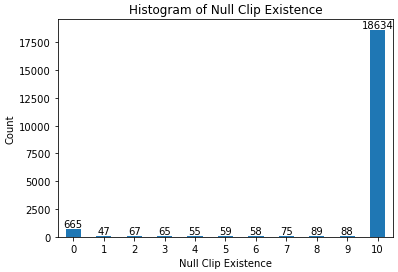
\includegraphics[width=0.5\linewidth]{null_clip_histogram.png}
    \caption{Distribution of null clips from the full 19,902 images downloaded.  Instances where less than 10 clips were taken are primarily due to the amount of urban area available in the satellite image.  There were three additional locations that were eventually able to provide 10 null clips, but not included before the dataset was finalized with 18,631 locations at training time.}
    \label{fig:null_hist}
\end{figure}






% Chapter Template

\chapter{Chapter Roadmaps} % Main chapter title
%this should end up being roughly 10 pages


\label{Chapter4} % Change X to a consecutive number; for referencing this chapter elsewhere, use \ref{ChapterX}

%----------------------------------------------------------------------------------------
%	SECTION 1
%----------------------------------------------------------------------------------------

\section{Dissertation Paper 1: Conflict prediction using Satellite Imagery}\label{sec:ch4_paper1}
In this chapter of my prospectus, I will outline each of my three dissertation papers, including my methods, data, and plans for implementation.  My first paper, presented here, is predicated upon the results from my quantitative study, as shown in chapter \ref{sec:chapter3}.  Because of overlap between my quantitative analysis and this paper, I provide a synopsis of each major stage of my work here, and refer you to chapter \ref{sec:chapter3} for a broader discussion.

\subsection{Major Research Question}
\textit{Can satellite imagery alone be used to determine the likelihood of conflict in urban areas?}

\subsection{Proposed Data \& Methods}
\subsubsection{Data}\label{sec:ch4_paper1_data}
Our full data processing pipeline is presented in section \ref{sec:data_paper1}, and briefly summarized here. In order to test this hypothesis, we first need to determine the locations where riots and protests occurred in the past. To accomplish this, we filter events from the full ACLED database using the following criteria: \textbf{1)} include riots and protests, \textbf{2)} an event with a known specific date, \textbf{3)} and events with a neighborhood-specific geographic footprint.  This criteria generates a list of 53,307 riots and protests.  We avoid over representing any single location, by only allowing locations to appear a maximum of 500 times.  This further filters our list of potential locations to 37,728 events.  

With this filtered list, we attempt to download satellite images of these 37,728 riots or protests.  Our strategy to download images is to search for satellite images from 24-48 hours prior to the riot or protest.  Also, we only consider images that contain 50\% or less cloud cover.  Under these constraints, we download 19,902 satellite images.  We will use these satellite images to construct our data set.

From each satellite image, we clip a 1 \textit{$\ km^{2}$} box centered on the latitude and longitude of the riot or protest.  We label these clipped images as "riot" in our data set.  The next task is to generate up to 10 null clips, each of which is a 1 \textit{$\ km^{2}$} box.  For each satellite image we use the following criteria: \textbf{1)} null clips must be a minimum of 10 km away from the riot, \textbf{2)} null clips must be from urban regions of the satellite image, \textbf{3)} null clips are spaced far enough apart, so that none of the null clip 1 \textit{$\ km^{2}$} boxes overlap.  We label these clipped images as "nulls" in our data set.

This generates a data set that consists of 1 \textit{$\ km^{2}$} boxes, that are labeled either "riot" or "null".  Specifically, the data set contains 18,631 "riot" images, and 186,310 "null" images.  In total, the data set has 204,941 images that we can use in training.


\subsubsection{Methods}
In order to determine the likelihood of a protest or riot, we train a ResNet18 convolutional neural network.  Starting with a pre-trained ResNet18, we can train the network to predict if clipped images are from riots/protests or from null locations.  Additionally, we explore the explainability of these clipped images using Score-CAM.  We also subset our data to explore any region or cultural patterns that might emerge in our analysis.   Our full implementation is discussed in section \ref{sec:methods_paper1}.


\subsection{Possible Challenges/Barriers}
During initial investigation into this topic, there were a few limitations that we encountered.  Some of these, such as explainabiliy limitations, have lead to future research areas.  I hope to explore many of these topics as a part of my broader dissertation.

\subsubsection{Satellite Information} \label{sec:limits.satinfo}
The satellite imagery we incorporated into this study had a number of notable limitations. First, while a satellite scene might contain 50\% or less cloud cover (see figure \ref{fig:cloudy_brazil}), the clipped images might be completely covered in clouds (see, for example, figure \ref{fig:cloudy_clips}).  Further, in some cases the conflict event selected may be at the edge of a scene, with no valid scene available to fill in null information, resulting in a partially clipped image (see figure \ref{fig:poorclips}).  Additionally, some of the clips contain interference or distortion, such as the clip at the bottom of figure \ref{fig:poorclips}.

Inter-related with these challenges, in many scenes we were unable to identify enough geographic locations to support the creation of 10 null cases. For example, in figure \ref{fig:coastline_clip} we can see that the riot location in consideration does not have any null location possibilities due to the riot's proximity to the coast, and the concomitant lack of proximate urban areas eligible for building null (no-protest) cases. There are similar limitations that cause the distribution of clipped images in figure \ref{fig:null_hist}.
\begin{figure}
    \centering
    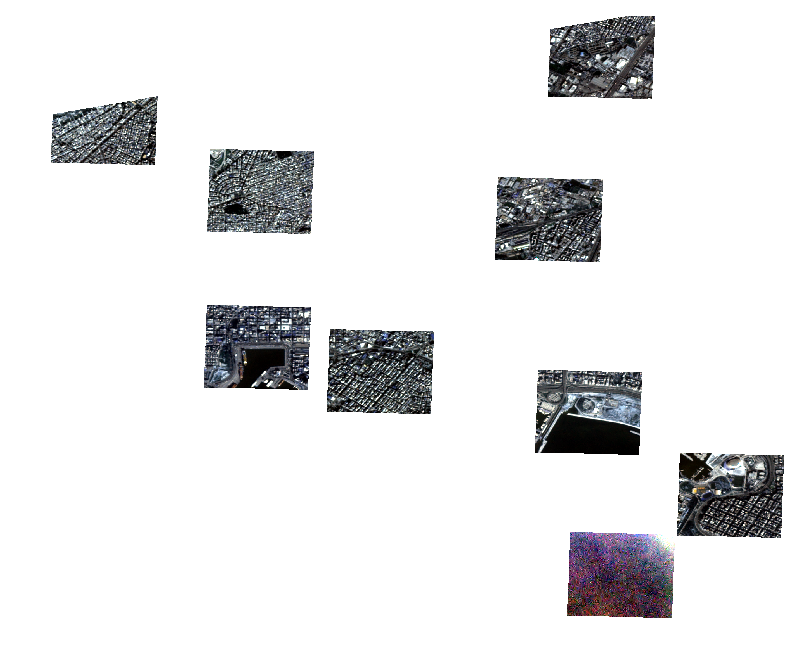
\includegraphics[width=0.5\linewidth]{poor_clips.png}
    \caption{9 of the null riot clipped images from Athens, Greece. Imagery \textcopyright Planet Labs PBC 2023. All rights reserved.}
    \label{fig:poorclips}
\end{figure}

\begin{figure}
    \centering
    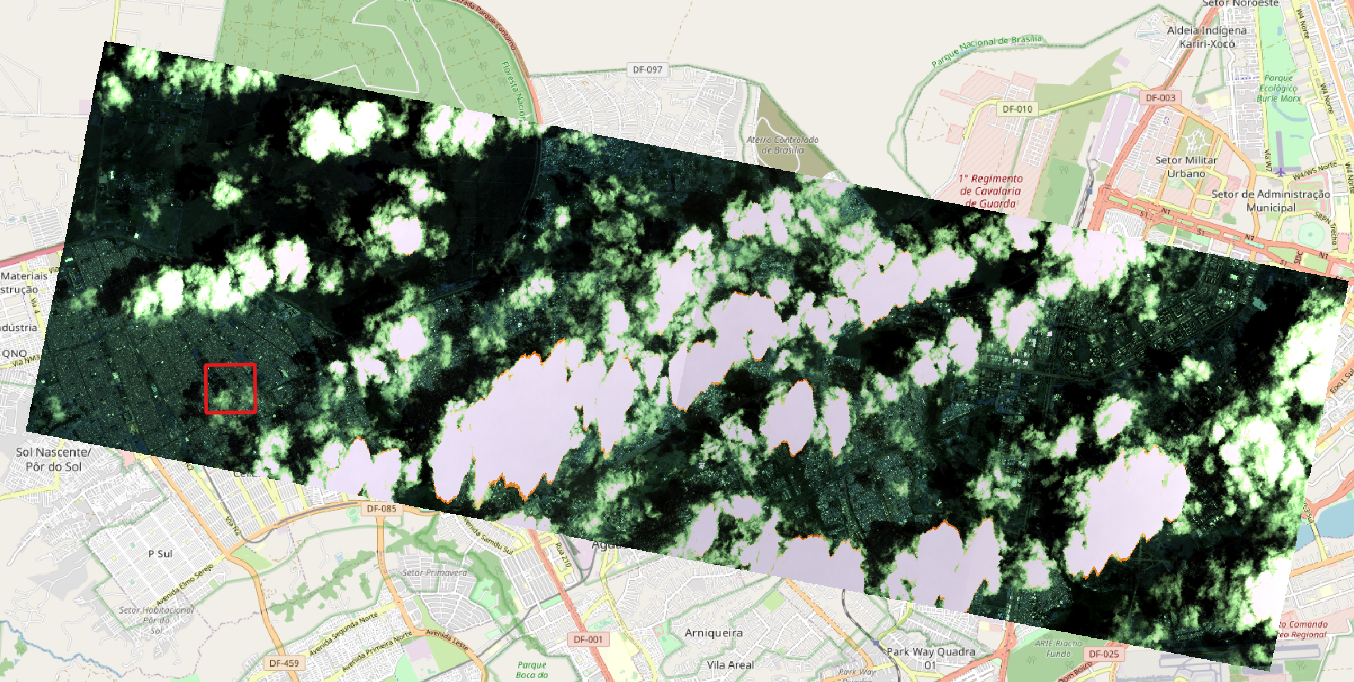
\includegraphics[width=0.75\linewidth]{cloudy_brazil.png}
    \caption{Satellite image of Brazil collected on 1 November 2018.  This image contains less than 50\% cloud cover for the full satellite scene.  The riot location indicated in the red square has minimal cloud cover, but other locations in the scene will be impacted by the cloud cover as seen in figure \ref{fig:cloudy_clips}. Imagery \textcopyright Planet Labs PBC 2023. All rights reserved.}
    \label{fig:cloudy_brazil}
\end{figure}

\begin{figure}
    \centering
    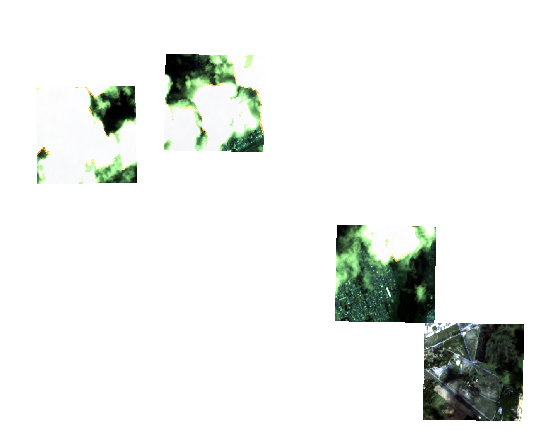
\includegraphics[width=0.5\linewidth]{cloudy_clips.png}
    \caption{Clips from a satellite image of Bazil collected on 1 November 2018.  While the full image contains less than 50\% cloud cover, many of the clips are partially or completely obscured. Imagery \textcopyright Planet Labs PBC 2023. All rights reserved.}
    \label{fig:cloudy_clips}
\end{figure}

\begin{figure}
    \centering
    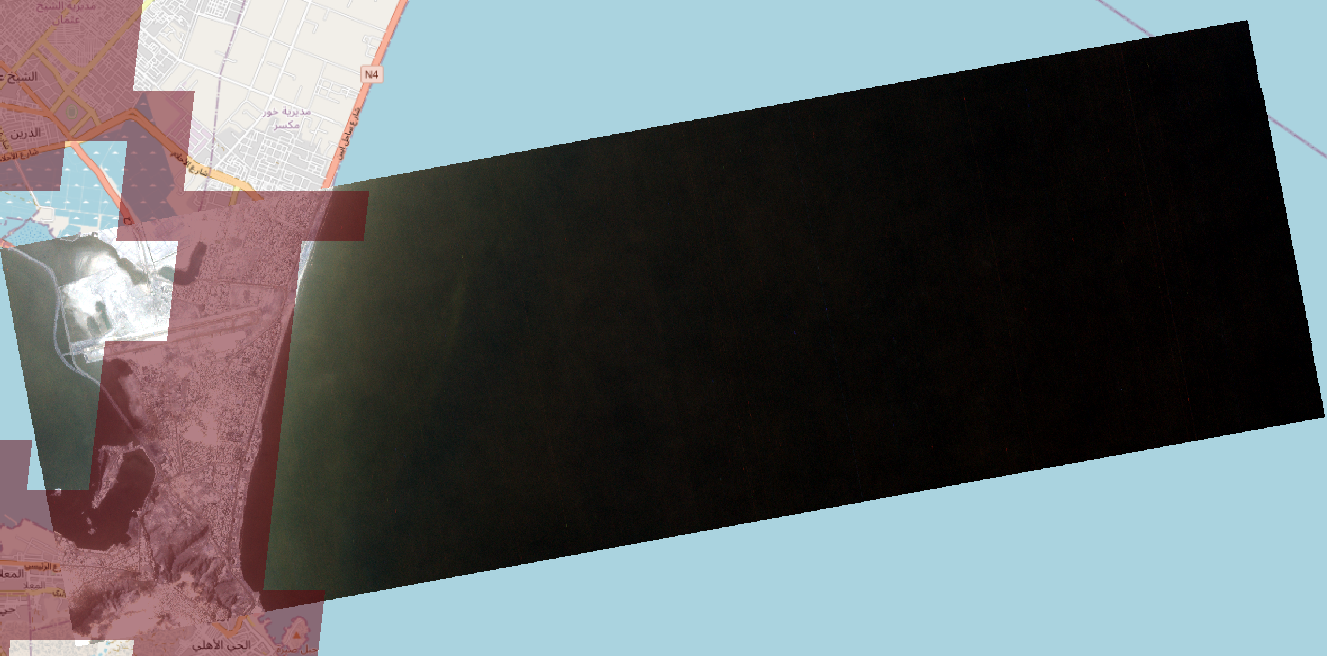
\includegraphics[width=0.75\linewidth]{coastline_clip.png}
    \caption{Satellite Image from Yemen collected on 14 September 2020.  The urban areas are shown in red.  Most of this image is not usable because of the lack of urban areas. Imagery \textcopyright Planet Labs PBC 2023. All rights reserved.}
    \label{fig:coastline_clip}
\end{figure}

Another limitation is in our definition of where conflict events occurred, as the definition of a ``neighborhood'' is inherently imprecise.  We used OpenStreetMaps \citep{OpenStreetMap2024} to visually compare the size of our ten most repeated locations \ref{tab:occurrence}.  We were able to confirm that the sizes of neighborhoods were inconsistent, but rarely of a size greater than our 10 square kilometer exclusionary zone (see figure \ref{fig:athens_nullclips}). 

To overcome this limitation, a future research direction might include ways to filter out clipped images with clouds or distortion.  Additionally if we only exclude clipped images within 1 km of the edge of the satellite scene, we could avoid images with only partial satellite information.  The neighborhood limitation is more difficult to account for, but we might group locations by their average neighborhood size and train the groups individually in an attempt to train our network to learn patterns that account for neighborhood size differences.

\begin{figure}
    \centering
    \begin{subfigure}[b]{0.45\linewidth}
        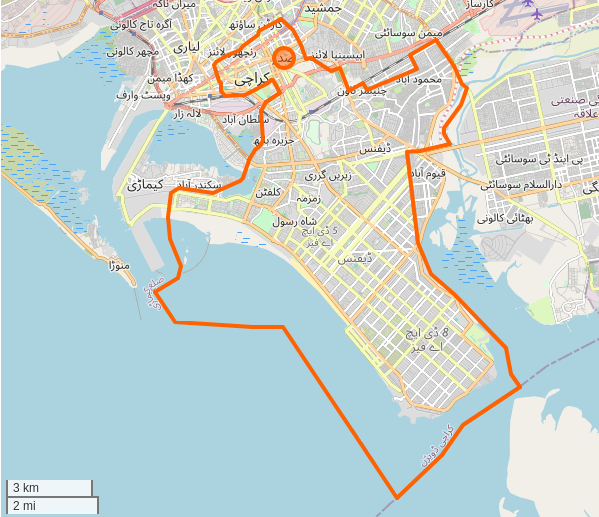
\includegraphics[width=\linewidth]{Karachi_Saddar.png}
        \caption{Karachi - Saddar }
    \end{subfigure}
    \quad 
    \begin{subfigure}[b]{0.45\linewidth}
        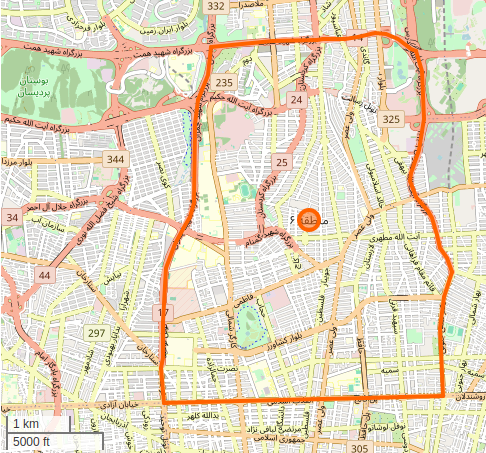
\includegraphics[width=\linewidth]{Tehran_District6.png}
        \caption{Tehran - District 6}
    \end{subfigure}
    \begin{subfigure}[b]{0.45\linewidth}
        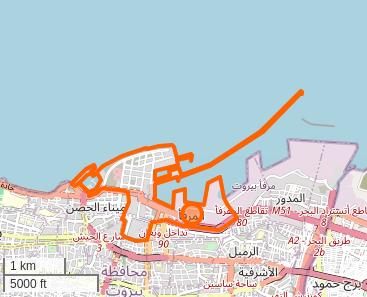
\includegraphics[width=\linewidth]{Beriut_Port.png}
        \caption{Beriut - Port}
    \end{subfigure}
    \quad 
    \begin{subfigure}[b]{0.45\linewidth}
        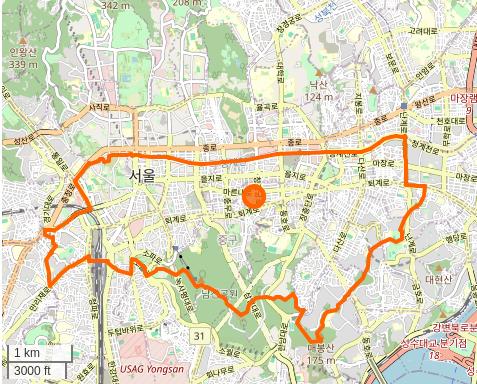
\includegraphics[width=\linewidth]{Seoul_Jung.png}
        \caption{Seoul - Jung}
    \end{subfigure}
    \caption{Four example neighborhoods from the top ten repeated locations.  The scale of the image is given in the lower left corner of each image. 
 The size of the neighborhoods is not consistent across the globe, but based of the labels in OpenStreetMap\citep{OpenStreetMap2024}, our methodology of excluding 10-km around the neighborhood will force our null cases to generate from locations outside the given neighborhood.}
 \label{fig:neighborhoods}
\end{figure}

\subsubsection{Explainability}\label{sec:explainability}
Currently, the majority of explainability techniques in the literature are focused on datasets consisting of object-centric images.  For example, two common data sets CIFAR-10 and CIFAR-100 \citep{cifar10_100} are used in many computer vision tasks and competitions, but those data sets only have objects centered in the middle of the picture, taking up most of the image space.  This differs significantly from our satellite imagery.  Our images contain all of the spatial information within a square kilometer in a city.  As opposed to an image of a cat or dog, our images have multiple buildings, cars, streets, parks, etc.  So while current explainability techniques can highlight portions of our image that lead to classification which are easily human interpretable, it is challenging for us to determine what in the image is being highlighted.  The example we discussed previously, sports stadiums, are identified in Score-CAM and easily identified visually in the satellite image.  There were other patterns that emerged in our Score-CAM analysis; however it is very difficult to describe many of the features Score-CAM identifies with easily identifiable semantic definitions. While we were able to identify a few other patterns, such as transitions from one zone to another zone (residential to commercial as an example), we are not confident in interpreting what these different types of zones are at this time.  The field of explainability, as it relates to satellite images, has very little published in literature and remains a strong avenue for future inquiry.

To overcome this limitation, a future research direction is outlined in section \ref{sec:paper_two}.  We intend to explore better understanding objects and spatial features identified by Score-CAM, through the use of points of interest identified in open source databases such as Overture Maps \citep{OvertureMapsFoundation2023}.  This would require segmenting the results of Score-CAM and comparing the objects indicated in Overture, to determine if there are patterns that arise indicating a riot or non-riot.  

\subsubsection{Additional Limitations}
There are a number of additional limitations of the presented work. 
 First, our data is focused on spatial information, not temporal, and thus we do not generate predictions of \textit{when} a riot will occur, only the likely urban locations.  Leveraging changes in images over time could help us overcome this challenge, but will necessitate new modeling strategies beyond those presented in this piece. Second, we have selected a ResNet18 as our base model, which could limit our model performance if alternative architectures are better performing. 

Third, the ACLED database used to construct our imagery data set is drawn primarily from news sources \citep{acled_codebook_2023}.  These comes with some inherent challenges and limitations.  If riots and protests are occurring in regions that traditional news sources are not reporting about, the events are not likely to populate the ACLED database.  Further, the nature of civil unrest is sometimes difficult to delineate with clear definitions, and different news organizations may cover a protest in conflicting ways - for example, a protest that is met with armed government resistance \citep{acled_codebook_2023}.  These challenges are not likely to be overcome in the near term, but are notable as they may impact the results presented in this study.

To overcome this limitation, a future research direction might include downloading new images from weeks or months before the riot, as well as images from after the riot date.  This would provide temporal differences for us to train our model to learn to differentiate.  We could do this with a ResNet, or attempt to train with alternate architectures.  To account for biases that might be present in the ACLED database, we might investigate alternate events within ALCED, or different databases.  


%----------------------------------------------------------------------------------------
%	SECTION 2
%----------------------------------------------------------------------------------------

\section{Dissertation Paper 2: Explainability in Satellite Imagery} \label{sec:paper_two}
While initial results from my first dissertation paper indicate that satellite imagery can be used to predict - with up to 97\% accuracy - where riots and protests are likely to occur in an urban area, it provides no insights into \textit{what features in the image are important}.  This is a critical step, as for policymakers to learn from or trust this model, we must understand the key on-the-ground factors that the model is leveraging. Thus, while my first chapter focused on the estimation of the location of a conflict event, in this chapter I will focus on explaining the features that were actually used.  


\subsection{Major Research Question}
\textit{Can we semantically describe the features within a satellite image that are consequential to the classification of urban conflict?}

\subsection{Data}
The core satellite imagery data used for this analysis will be the same dataset described in section \ref{sec:ch4_paper1_data}. This dataset provides over 2,178 images, which are each labeled as either a location at which protests or riots occurred, or an area drawn from the same urban environment at which no event occurred (see figure \ref{fig:athens_nullclips}).  Each of these images is a 1 \textit{$\ km^{2}$} box centered around a known riot/protest, or a non-riot location from the same satellite image as the riot clip. As a part of the quantitative analysis presented in Chapter \ref{sec:chapter3}, this data has already been acquired and processed. 

In addition to satellite imagery, this paper's activities will require a method through which the features that are identified as important on the ground are semantically labeled.  For example, a series of pixels that appears to represent a football stadium may be highlighted; in order to programmatically identify that location as a football stadium, we require a broad source of place names that we can correlate with the highlighted location. To accommodate this, we will leverage data sources from open source repositories, including SpaceNet\citep{SpaceNet}, DeepGlobe\citep{DeepGlobe2018}, xView\citep{xView}), Open Street Map \citep{OpenStreetMap2024}, and/or Overture Maps \citep{OvertureMapsFoundation2023}. All of these are open source and freely available, but at this time it is unknown which of these - or which combination of these - will be best suited for our purposes.

\subsection{Methods}
Our core aim is, given an image of a location and a deep learning model designed to estimate if conflict is likely to occur at that location or not, provide a human-understandable, semantic description of why the model made a given decision.  An output of this approach may be a sentence similar to one of these examples:\\
``It is likely that a riot will occur in this area, as it is proximate to numerous pubs and large public gathering spaces, in an area with a historic proclivity for riots.''\\
``It is unlikely that a riot will occur in this area, as there is a lack of large physical spaces in which crowds could aggregate.''\\
``We estimate, with 85\% confidence, that a riot is likely to occur in this area.  The key indicators included the presence of government properties and large fields in which aggregations can occur.''

In order to accomplish this, we propose a multiple-step process, in which:
\begin{enumerate} [itemsep=-1ex]
    \item We implement a modified Score-CAM (SAT-Cam) to capture the pixels which were important to the model's decision function.
    \item We threshold and then identify place names near the most important areas.
    \item We validate based on consensus between data sources and human labeled observations.
\end{enumerate}

\subsubsection{Step 1. Modified Score-CAM}
To date, explainability techniques in computer vision have predominantly emerged from traditional application - such as seeking to understand why an image taken from a cellphone is a cat or dog.  As noted in the introduction to this prospectus, this has resulted in a number of limitations when it comes to applications for satellite imagery-based analyses.  Critical themes include: \textbf{1.} Many current explainability techniques focus on images with a single object in the scene, satellite imagery by nature has many objects present in the same scene.  \textbf{2.} Satellite imagery will have less variance in pixel values when compared to other images used in computer vision tasks, which will make understanding which spatial features are important in classification challenging to decipher.  \textbf{3.} Semantic definitions are unclear in many satellite images, which will require us to use third-party data sources to distinguish features identified in explainability techniques.   

% \begin{enumerate} 
% \item \textbf{Multi-target limits} Many current explainability techniques in litureature focus on single objects \\
% \item Satellite imagery have significantly less variance in pixel values than other classes of data.\\
% \item Semantic definitions are unclear in many cases, forcing a reliance on third-party data sources.
% \end{enumerate}

In order to overcome these limits, we propose a modified implementation of Score-CAM.  Score CAM is a class activation map explainability method that utilizes weights as opposed to gradient in the model.  This method has demonstrated the ability to handle multi-target images better than other CAM methods \citep{wang2020score}.  It is formally defined as: 

\begin{equation}
\centering
L^{c}_{Score-CAM} = ReLU (\sum_{k} \alpha^{c}_{k} A^{k}_{l})  
\label{score-cam_equation}
\end{equation}
$\ A^{k}_{l} $ is the activation map for $\ k^{th} $ channel of layer \textit{l}, and $\ \alpha^{c}_{k} $ is the weight associated with the $\ k^{th} $ neuron. Where $\ \alpha^{c}_{k} = C(A^{k}_{l}) $ for convolutional layer \textit{l} and a class of interest \textit{c}. And $\ C(A^{k}_{l}) $ is the channel-wise increase of confidence introduced with Score-CAM.  \citep{wang2020score}.  

In order to overcome issues associated with multi-target limits and variance, we propose two changes to Score-CAM.  This revised algorithm, which we label "SAT-CAM", takes the following functional form:

\begin{equation}
L^{c}_{\text{SAT-CAM}} = \text{ReLU}\left(\sum_k \left\{
\begin{array}{cl}
\alpha_c^k A_k^l & \text{if } \alpha_c^k A_k^l > \epsilon \\
0 & \text{otherwise}
\end{array}
\right.\right)
\label{sat-cam_equation}
\end{equation}

Where $\ L^{c}_{SAT-CAM} $ is the output of SAT-CAM, that thresholds the Score-CAM evaluation $\ ReLU (\sum_{k} \alpha^{c}_{k} A^{k}_{l})$ by $\ \epsilon$.  In effect, this removes pixels below the threshold $\ \epsilon$ for consideration.

The output of SAT-Cam is a heat map matrix of the activation layer $\ A^{k}_{l} $ in which highlighted pixels contributed to the decision function.  Building on Score-CAM, $\ A^{k}_{l} $ is the last convolutional layer before the first fully connected layer.  This is passed into the next stage of the process, in which we seek to use ancillary geographic databases to semantically label the regions of the image that are identified as important.

\subsubsection{Step 2. Threshold \& Identifying Place-Names}

Using the output generated from SAT-CAM in equation \ref{sat-cam_equation}, we will apply a segmentation algorithm \citep{kirillov2023segment}, and then select the top 1 to 3 segments in terms of their absolute average value of importance.  Once selected, we will test three different approaches to semantic interpretation (two stand-alone approaches, and one integrated).  These are:
\begin{enumerate}
\item Clipping the underlying satellite imagery and passing it into an existing classification model. 
\item Identifying the place-names that are proximate to important areas from ancillary geospatial databases, and integrating them into a human-readable form. 
\item Providing both types of information into a large language model (LLM) to create a human-interpretable semantic description. 
\end{enumerate}


In the first approach, we seek to have a separate computer vision model label the isolated regions with their predominant structural characteristics.  For example, there are a number of challenges, SpaceNet Challenge \citep{SpaceNet}, DeepGlobe Challenge \citep{DeepGlobe2018}, and xView Detection Challenge \citep{xView}, that identify and label objects in satellite imagery.  This will leverage existing models, such as SpaceNet to decipher what objects are in the imagery.  If we apply these models to our regions of interest, we can generate a list of objects that appear frequently in our data.  By analyzing the results we might be able to determine what objects or spatial characteristics and features are critical in classification.

In the second approach, we will leverage data from sources such as Overture Maps \citep{OvertureMapsFoundation2023} and Open Street Map \citep{OpenStreetMap2024} to identify important place names proximate to the important features in geographic space.  First this will require construction of segments that contain the regions of interest identified in SAT-CAM.  These segments will have to be properly geo-referenced, so we only capture points of interest relevant to classification.  Using these segments as limiting constraints, we will then generate a list of the points on interest from Overture, as an example.  

These databases contain many types of information that might prove useful in explaining classification.  Overture Maps Foundation \citep{OvertureMapsFoundation2023}, for example, contains over 59 million locations.  Each location in the Overture map data contains not only location information (latitude and longitude), but also some class information, such as "residential", "commercial", or "education."  There are many land use classes as well, with examples such as "agriculture", "airport", "park", "recreation", "religious", and many more.  

This approach generates a list of location names, classes, and land uses for every segment identified by SAT-CAM.  Additionally, we have the classification of the overall image from the ResNet (riot or non-riot), the output of the final fully connected layer, and the accuracy of the classification (True Positive, False Negative, etc).  There is the potential to then leverage a LLM (Large Language Model) to help describe what is important in explaining classification.  A diagram displaying the data generation that will be used as input into the LLM is shown in figure \ref{fig:paper2_flowchart}.  At this point, all of the inputs would be text, and a trained LLM may be able to provide useful semantic descriptions given both the satellite-derived and gazetteer-based inputs.


\begin{figure}
    \centering
    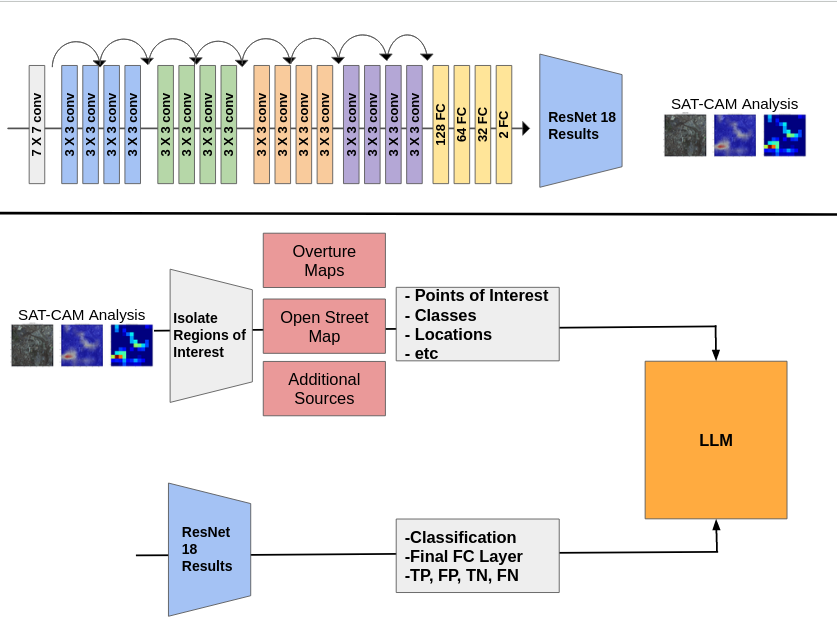
\includegraphics[width=0.75\linewidth]{Figures/paper2_data_flowchart.png}
    \caption{Flow chart detailing inputs into LLM.  We will use the outputs of our ResNet18 and SAT-CAM analysis to feed text into an LLM. }
    \label{fig:paper2_flowchart}
\end{figure}


A third approach, we will use a hybrid between the first two, in which a LLM will receive an input a prompt that contains all of the text input highlighted in the second approach (see figure \ref{fig:paper2_flowchart}) with the classification model utilized in the first approach.  This approach is more complicated, but leverages both the visual classification models that already exist and additional information about the segmented regions available in open source database.  

\subsubsection{Step 3. Validation}

There are two potential courses of action for validation of SAT-CAM, human labeling and consensus of databases.  The first viable option is to simply have individuals label by hand the relevant regions of interest and compare the human labels with the SAT-CAM labels.  This would be an relatively straightforward method when there is a single region of interest and a single human generated label.  However, as the number of regions of interest or the size of the regions increase, there will be an associated increase in the amount of data humans are required to label.  This increase spatial area has an accompanying increase in challenge and ambiguity.  For example, if half of a clipped image is categorized as important by SAT-CAM, half a square kilometer of an urban area must be labeled by a human.  Human labeling might prove easier to implement for smaller SAT-CAM results, and difficult to implement for large SAT-CAM results.

The second viable option for validation could be consensus.  The results of the SAT-CAM analysis require access to databases with labeled locations.  Once the methodology and data pipelines are established to evaluate a clipped image with SAT-CAM and generate a list of points of interest that exist within the segmented satellite data, the process can be replicated with different open source data bases.  If the list of locations for Overture Maps, Open Street Map, and potentially others, all agree, then the list is most likely an accurate representation of the spatial features important for classification.  



\subsection{Possible Challenges/Barriers}
There are a number of possible challenges to the successful execution of this work.  First and foremost is a lack of relevant past literature on which to build.  The majority of prior work in literature pertaining to computer vision uses data sets and examples that are object-centric.  Much of the prior work uses standard data sets such as CIFAR-10 and CIFAR-100, which consist exclusively of photographic images, with the object centered in frame.  Satellite imagery is very different in practice.  The dataset under examination in this study comprises satellite imagery, distinct from conventional photographs, encompassing spatial regions of interest that may appear at any location within the image frame, rather than being centrally positioned. This characteristic marks a significant departure from the datasets predominantly utilized in existing literature. 

Another potential challenge is that the Score-CAM results will contain both contiguous and non-contiguous results.  If all of the regions of interest are contiguous (as in figure \ref{fig:contiguous_ScoreCAM}), the association of the single region as the single entity that is important to classification is straight forward.  However, there are other Score-CAM results that are not contiguous (see figure \ref{fig:noncontiguous_ScoreCAM}), and it is unclear if these regions should be evaluated individually or collectively.  

Determining how to treat these non-contiguous areas as a non-overlapping polygons in the explainability research is similar to the object based image analysis (OBIA) challenge of analyzing images and objects at the appropriate resolution to avoid the "salt and pepper effect" \citep{blaschke2010object}.  So while there is similar work with satellite imagery, in fields such as OBIA, there is little work exploring the potential obstacles associated with explainability.  The non-contiguous nature of important features in satellite imagery could cause a number of challenges, opening a number of areas for inquiry.  Questions include: 
Is the classification determined by the sum of all weights or regions, or the maximum weight of a single region?
What role do interaction effects of non-contiguous regions play in classification?
Does the spatial distance between non-contiguous regions impact the classification of the image?
These challenges are specific to the use of explainability techniques in satellite images.

% \begin{figure}
%     \centering
%     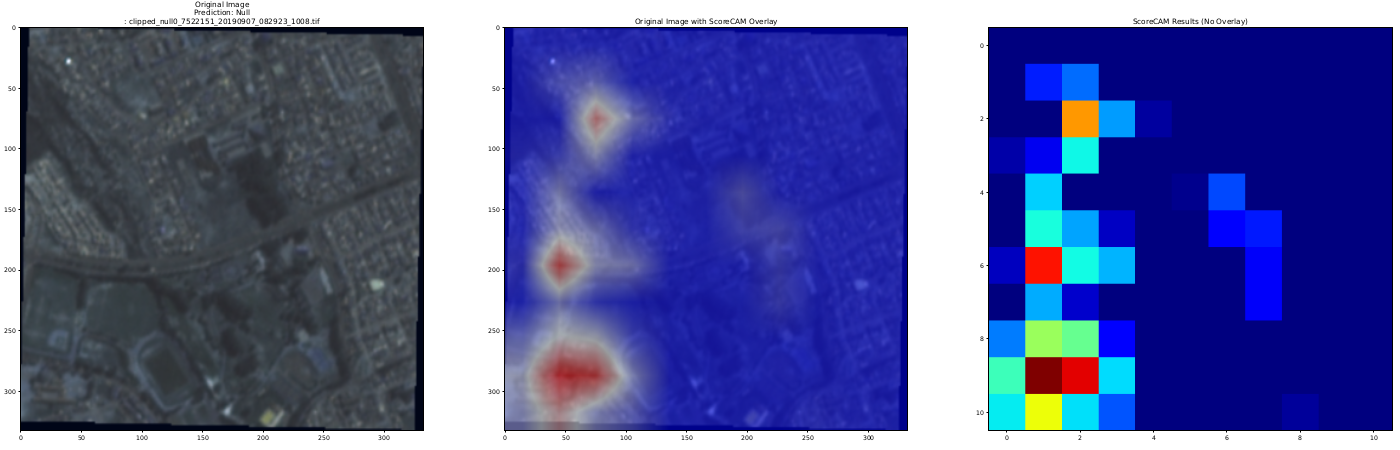
\includegraphics[width=1\linewidth]{stadium_scorecam2.png}
%     \caption{Example clipped image on the left.  The clipped image, a one kilometer box around a non riot location.  The Score-CAM overlayed on top of the image is shown in the middle.  The Score-CAM visual is displayed on the right }
%     \label{fig:score_cam_stadium2_ch4}
% \end{figure}

\begin{figure}
    \centering
    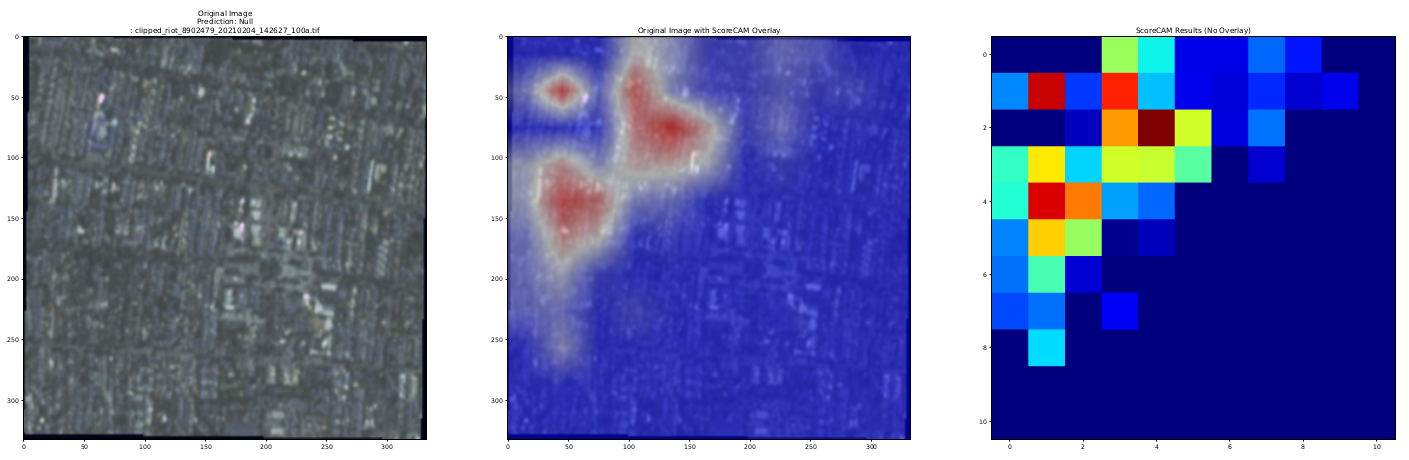
\includegraphics[width=0.75\linewidth]{contiguous_results.png}
    \caption{Score-CAM results displayed on the right of this figure represent a single contiguous region, regardless of the threshold set for consideration into a region of interest.}
    \label{fig:contiguous_ScoreCAM}
\end{figure}

\begin{figure}
    \centering
    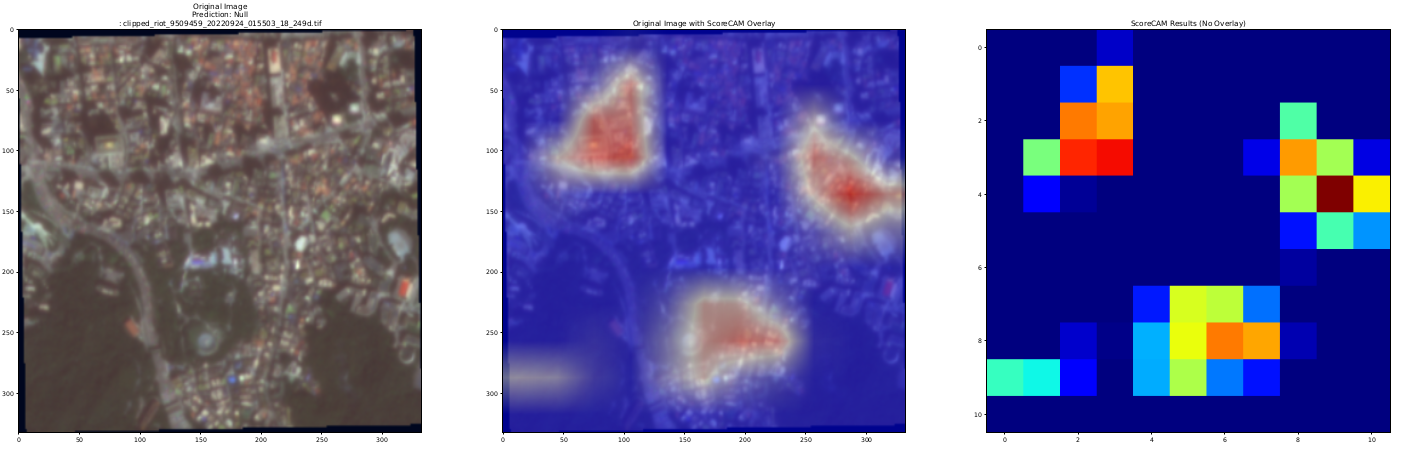
\includegraphics[width=0.75\linewidth]{noncontiguous_results.png}
    \caption{Score-CAM results displayed on the right of this figure represent a multiple regions of interest, regardless of the threshold set for consideration into a region of interest.}
    \label{fig:noncontiguous_ScoreCAM}
\end{figure}

%Another distinct issue that can arise with non-contiguous regions of interest, is if there are conflicts between classification.  When looking at non-contiguous results, such as the results in figure \ref{fig:noncontiguous_ScoreCAM}, it is possible that the region on interest in the upper left indicates one classification (i.e., a riot occurred), while the region in the upper right indicates a different classification (i.e., no riot occurred).   

Integral to the previously challenges is the underlying decision in determining what threshold to establish for consideration as a region of interest.  Before constructing the regions of interest, we must determine how much of the Score-CAM results should be used to consider.  If we set the threshold ($\ \epsilon $ in equation \ref{sat-cam_equation}) too low, we will consider too much of image.  If we consider too much of the image, the task of determining what in the image is being identified can be overwhelmed with too much non-essential information.  If we set the threshold$\ \epsilon$ too high, we will not consider enough of the image.  This will eliminate too much of the image, making identification, in terms of human interpretation, very challenging.  If we refer back to the sports stadium example discussed in Chapter \ref{sec:chapter3}, if we eliminate too much of the stadium because of a high threshold, we might only see some of the stadium making identification more challenging.



%----------------------------------------------------------------------------------------
%	SECTION 3
%----------------------------------------------------------------------------------------

\section{Dissertation Paper 3: Identification of conflict within Satellite Imagery }


\subsection{Major Research Question}
\textit{Can deep learning techniques enable the localization of conflict across a full-sized satellite image?}

While the first paper of my dissertation examines \textit{if} we can predict the likelihood of conflict using paired cases of images, and paper two explores \textit{why} these predictions are made, this leaves the question of if these tools can be operationally useful open.  While an algorithm that can discriminate between pairs of conflict and no-conflict cases may be useful, in practice it is unlikely that practitioners will have such a database.  More practically, they are likely to have many satellite scenes that they would like to identify probable locations of riots or protests.  While a model designed to take in pairs of images can accommodate this task, it requires additional modeling and testing in that broader context.  This chapter will fill that gap.

\subsubsection{Data}
My third paper will continue to leverage information from Planet, focusing on full images from the satellite sensors rather than clipped regions.  We plan to use the same source of data as specified in section \ref{sec:ch4_paper1_data}, which consists of 18,631 full satellite scenes distributed around the world. These images were collected from October 2017 to September 2022 and selected to be at least 24 hours prior to a conflict event.  An example of a single image collected from a satellite can be seen in figure \ref{fig:athens_baseimage}. 
 We also maintain a record of the latitude and longitude, as well as the clipped image, of the known riot for each full satellite scene.

%Our primary source of data is going to be the images we have previously downloaded.  These are full size satellite scenes of cities 24-48 hours prior to a known protest or riot.  Additionally we will use the pretrained ResNet18 from Chapter 3.   This network is trained to predict if a clipped 1-km box is from a riot or not from a riot.  

\subsubsection{Methods}
We will use our trained ResNet18 from chapter \ref{sec:chapter3} to identify the likely locations of riots and protests in full satellite scenes.  To accomplish this, we will take the following steps:
\begin{enumerate}
\item Create a grid that subsets the full satellite scene.
\item Systematically evaluate 1 $\ km^{2}$ boxes, encompassing the full satellite scene.
\item Collect results from step 2, to identify locations of probable riot or protest.
\end{enumerate}
In the first step of our methodology, we establish a grid that subsets the entire satellite scene into half kilometer boxes (see figure \ref{fig:grid_paper3}).  We subset the satellite scene, because we aim to evaluate the scene in a similar manner to a convolutional filter passing over a full image.  Our goal is to evaluate groups of subset half kilometer boxes in the same way a 2x2 convolutional filter captures the spatial relationship of four adjacent pixels in an input image, resulting in a single output value for the adjacent pixels.  We will evaluate four of the subset grids as a single clipped image and generate a single output, in our scenario a classification of riot or non-riot.  By subseting the full satellite scene into half kilometer boxes, we preserve the capability of our trained ResNet18 to evaluate each 2x2 grouping as an individual clipped image, similar to our data set in chapter \ref{sec:chapter3}.  This subseting of full satellite scenes will be unique to each individual scene.  As discussed in chapter \ref{sec:chapter3}, and highlighted in table \ref{tab:doves}, the spatial dimensions of images vary with each generation of satellite as well as the off-nadir angle from when the the image is captured.

\begin{figure}
    \centering
    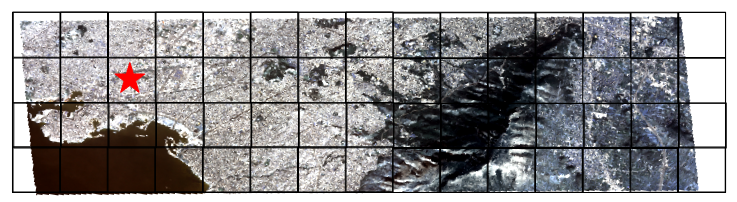
\includegraphics[width=0.75\linewidth]{Figures/grided_satimage.png}
    \caption{Example of grid that subsets entire satellite scene.  This image is not to scale, but represents a potential half kilometer grid that encompasses the full satellite scene.  In this example, there is a known feature(s) that causes a riot classification represented by a red star.  Imagery \textcopyright Planet Labs PBC 2023. All rights reserved.}
    \label{fig:grid_paper3}
\end{figure}

In the second step of our methodology, we evaluate the 2x2 adjacent half kilometer boxes across the full satellite scene.  Again, we build off the analogy of a convolutional filter sliding across an input image.  We will pad our satellite scene to account for data at the edge of the scene.  We implement a stride of one, to evaluate each half kilometer box multiple times.  An illustration of this process is shown in figure \ref{fig:eval_paper3}.  The purpose of subsetting the image and evaluating each half kilometer box as part of a 2x2 grouping, is to account for the unknown proximity relationship among spatial features that are important to riot classification.  This technique allows us to evaluate spatial features across a wider area of consideration, as opposed to limiting the spatial features to evaluation in the isolation of a single kilometer or half kilometer box. 

\begin{figure}
    \centering
    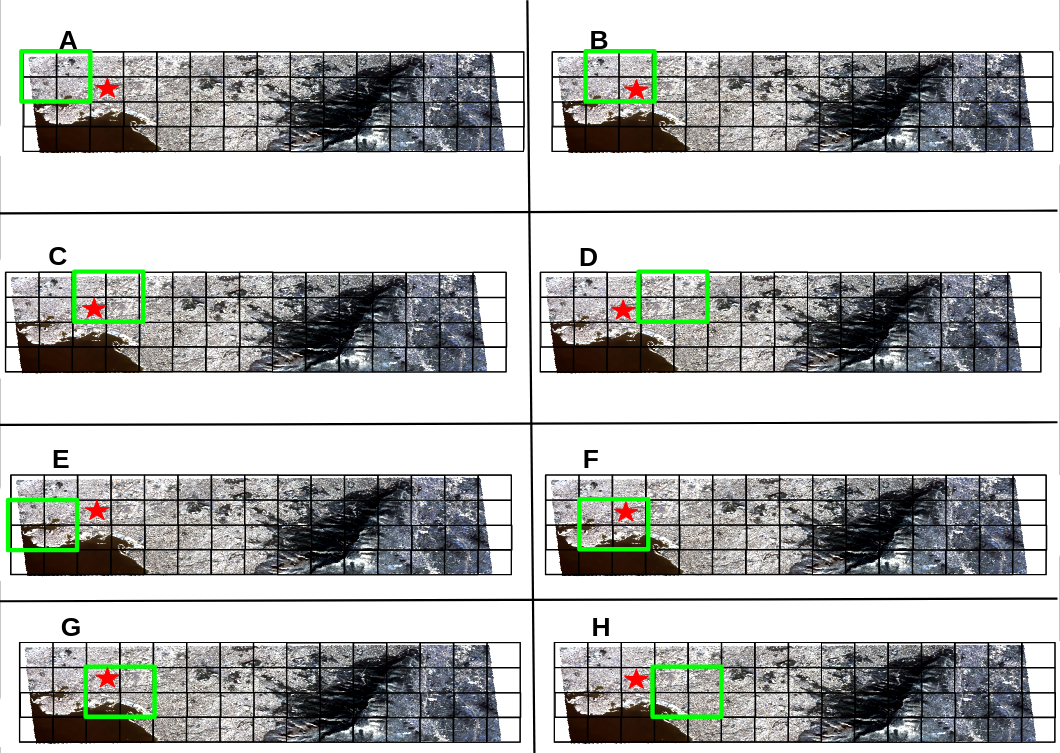
\includegraphics[width=1\linewidth]{Figures/eval_frames.png}
    \caption{This illustration is not to scale.  The green box represents the 2x2 convolutional filter used to evaluate the satellite scene.  Again, there is a known feature(s) that causes a riot classification represented by a red star.  The green box slides across the full scene.  In frames B, C, F, and G, all four of the half kilometer boxes would be marked as a riot.  In frames A, D, E, and H, none of the half kilometer boxes would be marked as a riot.  Imagery \textcopyright Planet Labs PBC 2023. All rights reserved.}
    \label{fig:eval_paper3}
\end{figure}

The third step is to collect the results of the second step to identify the probable locations for protests or riots.  Continuing with the 2x2 convolutional filter analogy, when the ResNet18 evaluates the four adjacent half kilometer boxes, all four are categorized as a riot or non-riot.  Each individual half kilometer box is evaluated four times, with different combinations of the surrounding boxes.  If the spatial features important to riot classification are present in a particular box, then that half kilometer box should be categorized as a riot four times.  While adjacent half kilometer boxes are categorized as a riot less than four times.  This will create a heat map across the full satellite scene, highlighting the particular regions in the image that are probable locations for riot or protest (see figure \ref{fig:heatmap_paper3}).  We then compare the heat map indicated locations to the known riot location to determine if the ResNet is able to determine the location of the riot or protest from a full satellite scene.

\begin{figure}
    \centering
    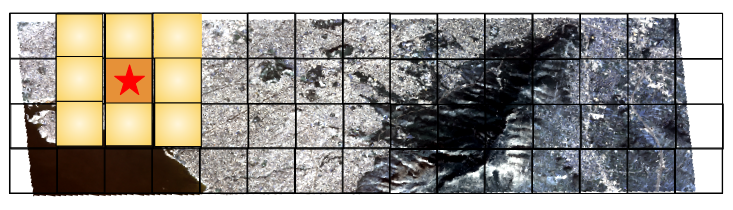
\includegraphics[width=0.75\linewidth]{Figures/heatmap_localized.png}
    \caption{The resulting heat map created during evaluation, that contains the spatial features that cause riot classification indicated by the red star.  Since the half kilometer box containing the red star was counted as a riot more often than its neighbors, this region appears as a hot spot that indicated probable riot or protest.  Illustration is not to scale.  Imagery \textcopyright Planet Labs PBC 2023. All rights reserved.}
    \label{fig:heatmap_paper3}
\end{figure}
There are two ways to validate our findings in step three.  The first is to measure the distance from the center of the region indicated in the heat map, to the latitude and longitude of the known riot.  The second is to compare how much the clipped image overlaps with the hot spots from the heat map.  It is currently unknown if our outlined methodology will result in the identification of a single riot or multiple riots.  We also do not know the size of any of the hot spots our methodology will create.  We are currently exploring the most appropriate manner for evaluation of performance in terms of accuracy, precision, recall, or other relevant measures.

There is potential to include further analysis related to explainability highlighted in section \ref{sec:paper_two}.  After identifying regions in the full image that are likely to have a protest, we can implement SAT-CAM to gain insight into the features driving classification.  It is currently unknown how the relationship between spatial features and their distribution impact classification.  Additionally, we do not know how spatial separation among important features influences classification across wider areas, such as full satellite scenes.  For example, large parks and the presence of government buildings might drive riot classification in a single one kilometer clipped image, but those same features when separated by a greater distance might no longer indicate a riot.


\subsection{Possible Challenges/Barriers}
There are a few potential challenges with this methodology.  One of the key assumptions in our training data is that there is only one riot or protest in each satellite scene, or at least there are no riots outside the ten kilometer exclusion area when the null clips were created (as described in chapter \ref{sec:chapter3}).  If there are other riots in the satellite scene, the trained network might correctly identify riot locations outside the known clip location, and based on our training data we would consider that a miss-classification.  

Another potential challenge identified for this study involves the methodology of analyzing entire satellite scenes to detect instances of riots or protests using a network originally trained on one-square-kilometer segments. The underlying assumption of our model posits that the spatial characteristics relevant to the classification task are less than one kilometer in size and that any spatial correlations critical for accurate classification occur within this distance. However, this assumption may not hold in all cases, as it is conceivable that certain spatial features or indicators of a riot or protest exceed this size limit or are dispersed beyond a kilometer, leading to potential inaccuracies in classification. This challenge underscores the need for a robust evaluation of the model's assumptions and its capability to generalize across varying spatial dimensions.

A further potential challenge originates from parameter choice in our methodology.  We opt for a half kilometer segmentation in order to evaluate each half kilometer box multiple times with its adjacent neighbors.  While this allows each segment to be classified multiple times, we might not be isolating the relevant spatial features enough.  We could attempt to compensate for this by decreasing the size of our grid.  For example we could use a quarter kilometer grid, and include a filter with a 4 x 4 block to construct a kilometer box for evaluation.  This would allow us to evaluate the relevant spatial feature more often, but it would also increase the computational cost.  We do not know the size of the features that are relevant to prediction, nor do we know if they are consistent in size.  So we are presented with an unknown constraint to the appropriate size of the grid to best capture the relevant features.  This problem is similar to the issue of required spatial resolution for object based image analysis \citep{blaschke2010object}







% Chapter Template

\chapter{Timeline for Degree Completion} % Main chapter title
%this should end up being roughly 2-3 pages
\label{Chapter5} % Change X to a consecutive number; for referencing this chapter elsewhere, use \ref{ChapterX}



\section{Gaant Chart}
The work described in my quantitative section, chapter \ref{sec:chapter3} and section \ref{sec:ch4_paper1} was submitted to \textit{Transactions in Geographic Information Science} on 15 March 2024, and is currently under review (shown in blue in figure \ref{monthly_gantt_chart}).  This is important in subsequent phases of my dissertation.  This initial research is responsible for generating a significant portion of the data required for follow on phases.  This included the selection, download, and pre-processing of over 4 TB of satellite imagery data. The amount of work invested in constructing this data set, should facilitate the ambitious timeline I present to support a May 2025 graduation (see figure \ref{monthly_gantt_chart}). 

Specifically, the first paper included preliminary work into explainability in satellite imagery.  The goal of the second phase of the research (purple in figure \ref{monthly_gantt_chart}) is to identify specific features in the image that might be important in classification of the image as either a riot or not.  The first two tasks in this are to gather point of interest data from Overture Maps \citep{OvertureMapsFoundation2023}, and to segment the pixels of interest from the Score-CAM analysis.  These two tasks can be accomplished concurrently during the month of April, given current progress.  During May, I will work on an algorithm which integrates points of interest with the pixels of interest to determine patterns of physical features on the ground that the trained ResNet has learned to associate with riots or null riots.  A goal of completing this phase by the summer of 2024, should be attainable and provide a much richer understanding of explainability as it pertains to satellite imagery.

The third chapter of my dissertation (orange in figure \ref{monthly_gantt_chart}) involves identifying conflict from contiguous satellite images, contrasted with classification of smaller 1\textit{$\ km^{2}$} boxes in the first phase.  The first task in this phase is to determine the appropriate methodology to segment full satellite images into a grid for subsequent conflict searches.  This effort should begin in July 2024.  By August, I will be training neural networks to detect riots within these full satellite scenes.  This will likely result in refinement in either the grid segmentation of satellite scenes, or the training of neural networks.  Depending on the initial results of this, there is a potential that I will have to increase the volume of my current data set or alter my methodology.  My current plan is to be complete with this research effort by the end of 2024.


I propose the following anticipated timeline, with consideration given to the dissertation milestones (indicated in green in Figure \ref{monthly_gantt_chart}), which are aligned to support a graduation in May 2025. In my initial paper, I aim to contribute to the body of literature on deep learning, conflict, and the classification of satellite imagery in urban environments. Subsequently, my second paper will delve into novel areas of explainability within the context of satellite imagery. Lastly, in my third paper, I plan to broaden the scope of my research by extending the functionality from analyzing small urban areas to encompassing comprehensive satellite scenes of larger areas.



\begin{figure}
    \centering
    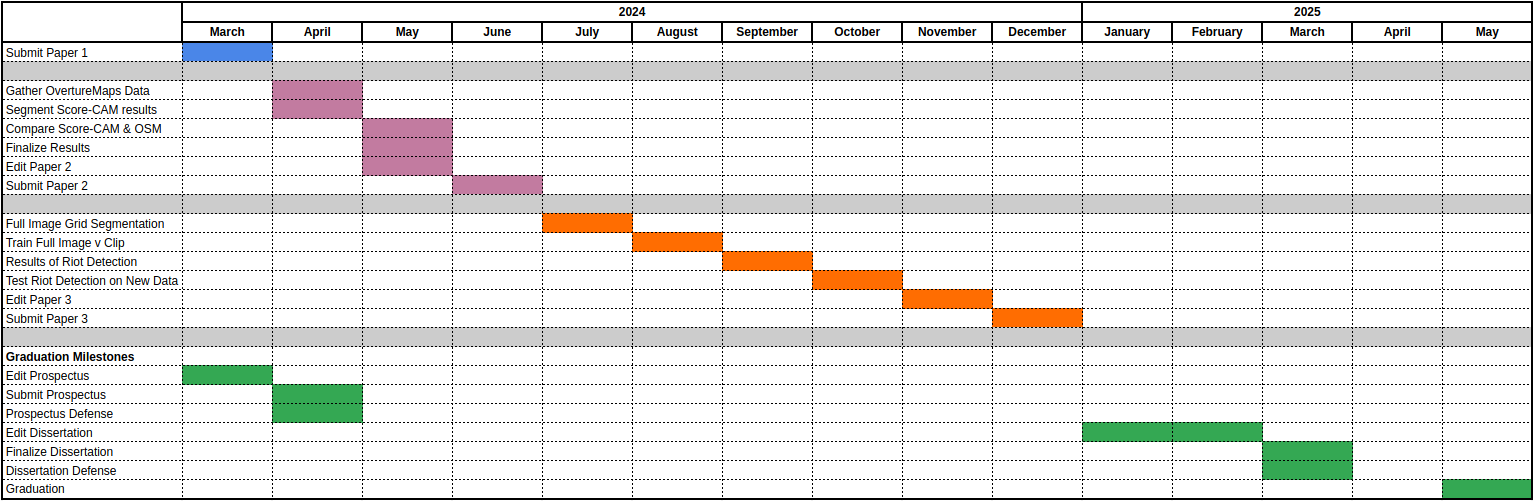
\includegraphics[width=1\linewidth]{Figures/monthly_gantt_chart.png}
    \caption{Gantt Chart supporting a May 2025 graduation. }
    \label{monthly_gantt_chart}
\end{figure}




% % Chapter Template

\chapter{Timeline for Degree Completion} % Main chapter title
%this should end up being roughly 2-3 pages
\label{Chapter5} % Change X to a consecutive number; for referencing this chapter elsewhere, use \ref{ChapterX}



\section{Gaant Chart}
The work described in my quantitative section, chapter \ref{sec:chapter3} and section \ref{sec:ch4_paper1} was submitted to \textit{Transactions in Geographic Information Science} on 15 March 2024, and is currently under review (shown in blue in figure \ref{monthly_gantt_chart}).  This is important in subsequent phases of my dissertation.  This initial research is responsible for generating a significant portion of the data required for follow on phases.  This included the selection, download, and pre-processing of over 4 TB of satellite imagery data. The amount of work invested in constructing this data set, should facilitate the ambitious timeline I present to support a May 2025 graduation (see figure \ref{monthly_gantt_chart}). 

Specifically, the first paper included preliminary work into explainability in satellite imagery.  The goal of the second phase of the research (purple in figure \ref{monthly_gantt_chart}) is to identify specific features in the image that might be important in classification of the image as either a riot or not.  The first two tasks in this are to gather point of interest data from Overture Maps \citep{OvertureMapsFoundation2023}, and to segment the pixels of interest from the Score-CAM analysis.  These two tasks can be accomplished concurrently during the month of April, given current progress.  During May, I will work on an algorithm which integrates points of interest with the pixels of interest to determine patterns of physical features on the ground that the trained ResNet has learned to associate with riots or null riots.  A goal of completing this phase by the summer of 2024, should be attainable and provide a much richer understanding of explainability as it pertains to satellite imagery.

The third chapter of my dissertation (orange in figure \ref{monthly_gantt_chart}) involves identifying conflict from contiguous satellite images, contrasted with classification of smaller 1\textit{$\ km^{2}$} boxes in the first phase.  The first task in this phase is to determine the appropriate methodology to segment full satellite images into a grid for subsequent conflict searches.  This effort should begin in July 2024.  By August, I will be training neural networks to detect riots within these full satellite scenes.  This will likely result in refinement in either the grid segmentation of satellite scenes, or the training of neural networks.  Depending on the initial results of this, there is a potential that I will have to increase the volume of my current data set or alter my methodology.  My current plan is to be complete with this research effort by the end of 2024.


I propose the following anticipated timeline, with consideration given to the dissertation milestones (indicated in green in Figure \ref{monthly_gantt_chart}), which are aligned to support a graduation in May 2025. In my initial paper, I aim to contribute to the body of literature on deep learning, conflict, and the classification of satellite imagery in urban environments. Subsequently, my second paper will delve into novel areas of explainability within the context of satellite imagery. Lastly, in my third paper, I plan to broaden the scope of my research by extending the functionality from analyzing small urban areas to encompassing comprehensive satellite scenes of larger areas.



\begin{figure}
    \centering
    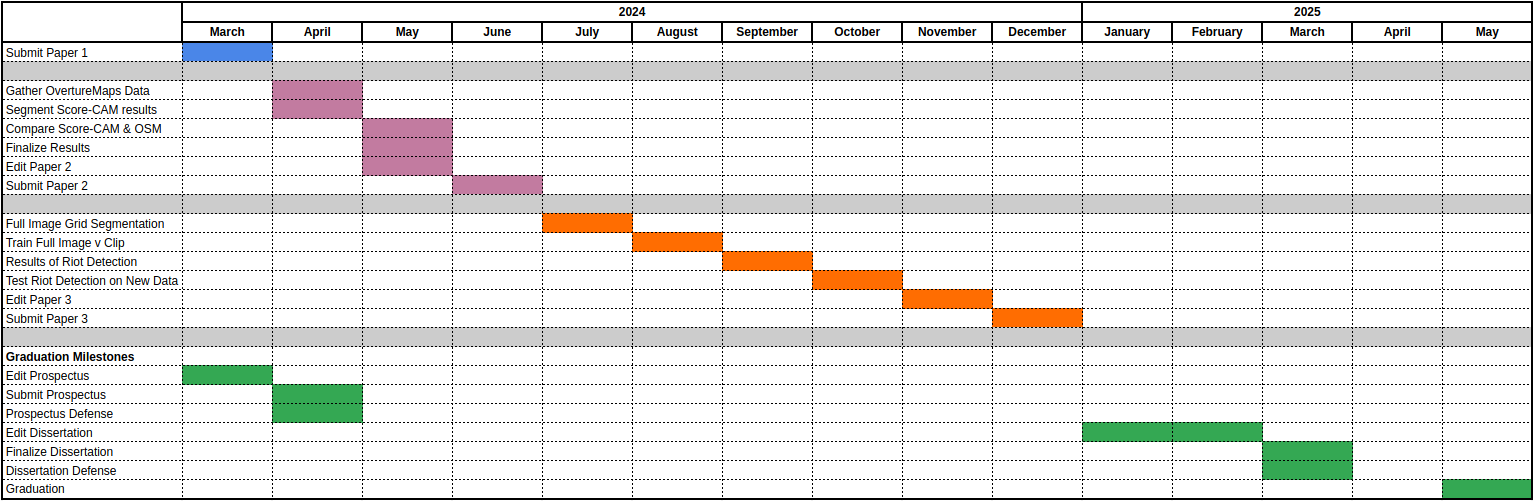
\includegraphics[width=1\linewidth]{Figures/monthly_gantt_chart.png}
    \caption{Gantt Chart supporting a May 2025 graduation. }
    \label{monthly_gantt_chart}
\end{figure}

 

% \include{Chapters/Tutorial}

%----------------------------------------------------------------------------------------
%	THESIS CONTENT - APPENDICES
%----------------------------------------------------------------------------------------

\appendix % Cue to tell LaTeX that the following "chapters" are Appendices

% Include the appendices of the thesis as separate files from the Appendices folder
% Uncomment the lines as you write the Appendices

% % Appendix A

\chapter{Frequently Asked Questions} % Main appendix title

\label{AppendixA} % For referencing this appendix elsewhere, use \ref{AppendixA}

\section{How do I change the colors of links?}

The color of links can be changed to your liking using:

{\small\verb!\hypersetup{urlcolor=red}!}, or

{\small\verb!\hypersetup{citecolor=green}!}, or

{\small\verb!\hypersetup{allcolor=blue}!}.

\noindent If you want to completely hide the links, you can use:

{\small\verb!\hypersetup{allcolors=.}!}, or even better: 

{\small\verb!\hypersetup{hidelinks}!}.

\noindent If you want to have obvious links in the PDF but not the printed text, use:

{\small\verb!\hypersetup{colorlinks=false}!}.

%\include{Appendices/AppendixB}
%\include{Appendices/AppendixC}

%----------------------------------------------------------------------------------------
%	BIBLIOGRAPHY
%----------------------------------------------------------------------------------------

\printbibliography[heading=bibintoc]


%----------------------------------------------------------------------------------------

\end{document}  
